\chapter{Results}\label{ch:results} 

This chapter discusses the results comparing the compatibility of the observed data with the background-only versus various signal-plus-background hypotheses using a shape-based Bayesian Marginalization procedure for the ADD Large Extra Dimensions and the Clockwork model. The Unparticles model uses a simpler cut-and-count approach rather than a shape-based analysis for the preliminary investigation.

% In the Section~\ref{sec:expected_sensitivity}, we show the expected limits results using pseudodata. These results were obtained prior to unblinding in the signal region $\mgg > 1000$~GeV. In Section~\ref{sec:observed_results}, we perform the unblinding and show the observed limits. 

\section{\label{sec:bayesian_inference} Bayesian Confidence Intervals}

We use a bayesian inference technique to set upper limits on the ADD Large Extra Dimensions and the Clockwork Signal model using the \texttt{THETA} framework~\cite{THETAFrameworkIntro}. The framework uses the Markov-Chain Monte Carlo (MCMC) method to marginalize or integrate out the nuisance parameters to obtain the posterior distribution for the signal strength that can be integrated to arrive at the 95\% CL exclusion limit.

Given some prior degree of belief in a hypothesis $A$ for an experimental measurement, the probability for a given event to occur can be inferred through Bayes' theorem:

\begin{equation} \label{eq:Bayestheorem}
P(A|B) = \frac{P(B|A)P(A)}{P(B)}.
\end{equation}

Here, $P(A|B)$ is the posterior probability of the hypothesis A given B, which in this case is the data. $P(B|A)$ is the called the "marginal likelihood" which indicates the probability of the event/data being true, given A. $P(A)$ corresponds to our knowledge, or what is called the \textit{prior}, which is the measure of the probability of A being true.  $P(B)$, is the marginal likelihood, which is the probability of the data being true. For this limit-setting procedure, we construct a binned likelihood such that the total likelihood $\mathcal{L}$ is equal to the product of the individual likelihoods $\mathcal{L}_{i}$ in each bin $i$. Since we count the number of events occuring in each bin, the likelihood in each bin can be written using the Poisson Distribution formula,

\begin{equation} \label{eq:poisson_likelihood}
\mathcal{L}(N| \mu_i ) = \prod_{i} \mathcal{L}_{i}(N_i | \mu_i ) = \prod_{i} \frac{\mu_i^{N_i} e^{-(\mu_i)}}{N_i!},
\end{equation}

where the index $i$ runs over all the bins of the histogram. $N_i$ is the number events in the bin $i$ and $\mu_i$ is the sum of the signal strength $
\beta$ times the number of signal events in bin $i$ plus the number of background events $b_i$ in the same bin:

\begin{equation} \label{eq:splusb}
\mu_i = \beta s_{i} + b_i.
\end{equation}

We can now rewrite Eq.~\ref{eq:Bayestheorem} as follows,

\begin{equation} \label{eq:posterior}
P(\beta, N) = \frac{\mathcal{L}(N_i| \mu_{i} (\beta) \pi(\beta)}{P(N)} = \mathcal{L}(N_i| \mu_i) \pi(\mu_i).
\end{equation}

Here, $P(N)$ is treated as a normalization constant that has been absorbed into the likelihood. We see here that the posterior is proportional to the likelihood.

Both the signal and background have associated systematic uncertainties that affect our knowledge of their associated yields. We assign a separate nuisance parameter $\theta$ for each of these systematic uncertainties which are detailed in Table~\ref{tab:Systematics}. For each of these nuisance parameters, a different choice of prior $\pi(s,b, \theta)$ is made. These constraints allow the signal and background yields to deviate from their nominal values, subject to some cost or penalty on the likelihood in the form of a normal or lognormal distribution. These  individual parameters are described in Sec.~\ref{ch:systematics}. They are either assumed to be fully correlated across the $\mgg$ bins across all the 6 signal regions, i.e. the 3 years for BB and BE. Otherwise, separate nuisance parameters are used for each signal region. 

The $\mgg$ distributions for both the signal and the background are binned in 100 GeV steps from 500 GeV. These, together with the nuisance parameters and additional shape-based uncertainties are extracted from \texttt{root} files to construct the statistical model. The framework then performs a maximum likelihood fit to get estimates for all model parameters. At this step the nuisance parameters are simultaneously marginalized, and a posterior prediction for the combined prompt plus fake ($\gamma\gamma$ + $\gj$) $\mgg$ distribution is produced using the data as a constraint. By convention in particle physics, a flat prior $\pi(\beta)$ with a lower bound of 0 is given for the signal strength. This is motivated by our lack of prior knowledge on its uncertainty and the fact that this is a shape analysis. It is often considered a good choice due to simplicity, ease of implementation, and it provides a more objective approach since it avoids the introduction of additional assumption in the analysis. The other nuisance parameters accounting for the associated systematic uncertainties for the signal and background are marginalized or integrated out as follows:


\begin{equation}
    P(\beta |N) = \int P(\beta \theta |N_i) d\theta = \int \mathcal{L}(n| \beta, \theta) \pi(\beta,\theta) d\theta, 
\end{equation}

where  $\pi(s,b, \theta)$ is the chosen prior for each nuisance parameter. To determine the 95\% upper limits on the signal, we need to integrate the posterior prediction to 95\% of the total integral.

\begin{equation}\label{95CL}
   \int^{\beta}_0 P(\beta |N)  = 0.95\times\int^{\infty}_0 P(\beta |N). 
\end{equation}

\section{Exclusion Limits: ADD and Clockwork}~\label{sec:ADDCWresults}

% This section presents the results of the non-resonant search which, \ie{}, the data over the background at prefit and postfit estimates, 
% as well as the interpretation of the results to physics beyond the SM. 

% In Figure~\ref{fig:Prefit_spectra}, we show the out-of-the-box SHERPA SM prompt $\gamma\gamma$ diphoton prediction reweighted by the NNLO k-factor correction, the fake $\gj$ background and the unblinded data. In the signal region above $\mgg > 1$ TeV which is also the range of high sensitivity, the fake background constitutes only 5\%(15\%) for BB (BE) channels. The bottom pads present the "pulls" ( $(\textrm{Data - Pred})/\sigma_{STAT}$) which describe the consistency between data and the MC prediction and the orange bands present the prefit rate systematic uncertainties for the real $\gamma\gamma$ (5\%) and the fake $\gj$ uncertainties (30\%) (See Table~\ref{tab:Systematics}. A fairly good agreement is observed between the prediction within the systematic uncertainties save for some bins which are slightly off the $\pm 1\sigma$ uncertainty band. One thing to note is that these predictions aren't the final prediction of the total SM background. Instead the final prediction would come from the post-fit distributions where the nuisances have been marginalized together with the signal strength. 
\subsection{Prefit Prediction}~\label{sec:Prefit}
The unblinded \mgg spectra are shown at Figs.~\ref{fig:Prefit_spectra2016},~\ref{fig:Prefit_spectra2017}, and~\ref{fig:Prefit_spectra2018} together with the prefit prediction. The prediction of real \gmgm background and the fake $\gj,jj$ background are shown in light and dark filled histograms respectively.
We observe that the fake background, in the range of high sensitivity $\mgg>1\TeV$, amounts approximately only 5\% (15\%) for BB (BE) channels. 
The bottom pads present the pulls - the difference between the data and the MC prediction divided by the standard deviation $\sigma_{STAT}$, as well as the magnitude of prefit rate systematic uncertainty, $\sigma_{SYS}$, where for the latter only the 5\% of real and the 30\% of the fake backgrounds uncertainties on rate have been considered.
The data exhibit over all a fair agreement with the prefit background estimate withing the systematics uncertainties, while in some case (for low masses) the data are slightly off the $\pm1\sigma$ uncertainty band for a few sequential bins. The spectra are fit within the range of 500--4000 \GeV, were the last bin includes the overflow events. Additionally, the \mgg background normalization is allowed to float freely within 5\% in the BB and BE categories separately. The low-mass data will easily constrain the nuisance parameters.

\begin{figure}[!htbp]{\centering{
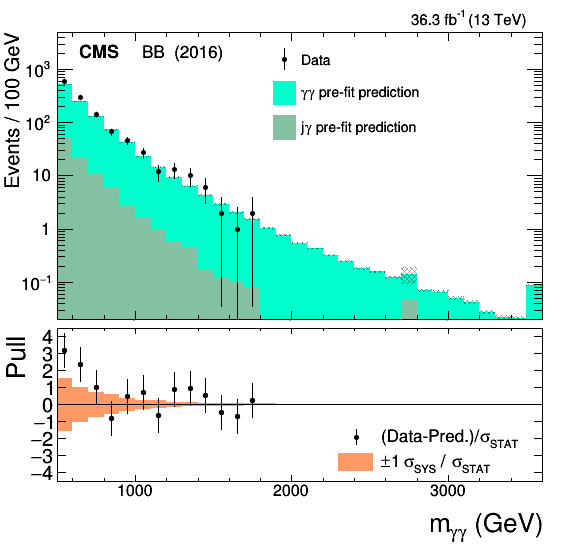
\includegraphics[width=0.49\textwidth]{fig/PLOT_PRED_PULL_BB16_6000_ADDGRW_0_0.png}
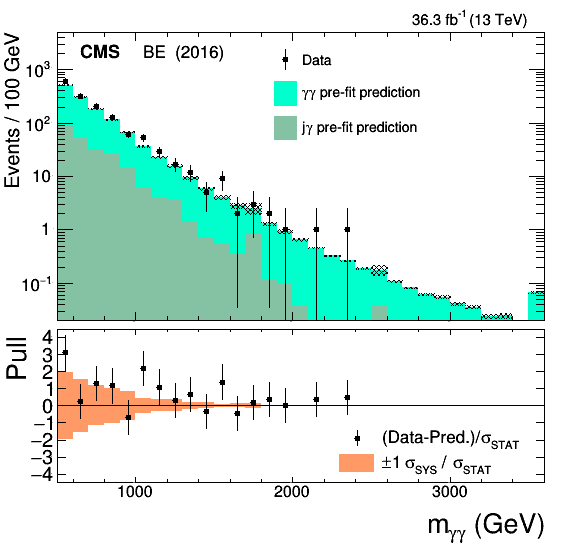
\includegraphics[width=0.49\textwidth]{fig/PLOT_PRED_PULL_BE16_6000_ADDGRW_0_0.png}
% 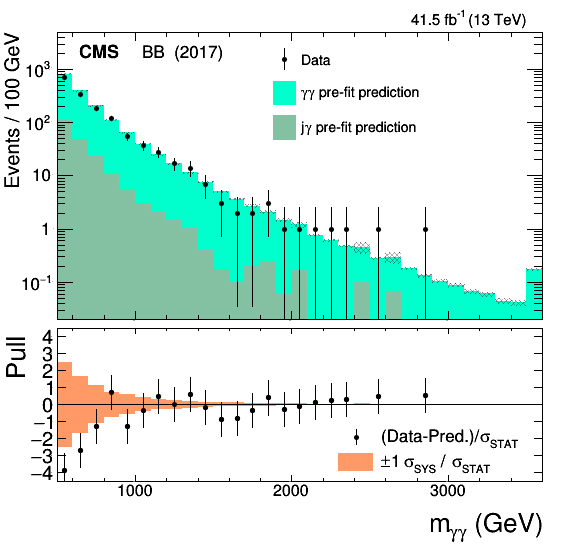
\includegraphics[width=0.49\textwidth]{fig/PLOT_PRED_PULL_BB17_6000_ADDGRW_0_0.png}
% 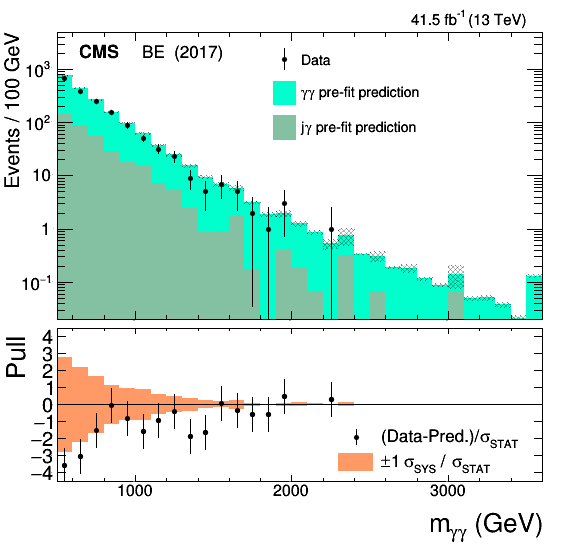
\includegraphics[width=0.49\textwidth]{fig/PLOT_PRED_PULL_BE17_6000_ADDGRW_0_0.png}
% 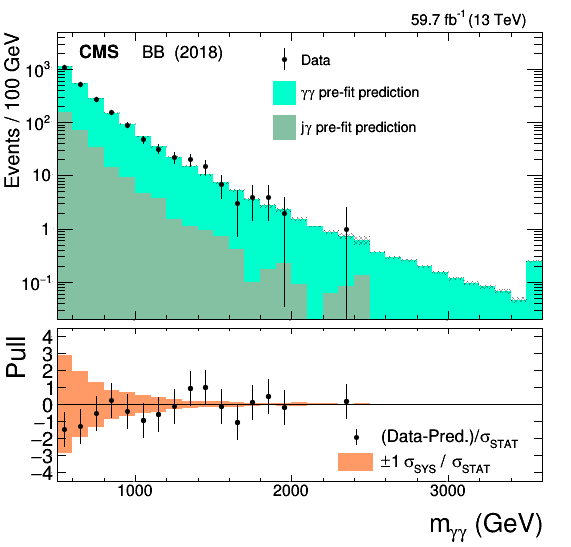
\includegraphics[width=0.49\textwidth]{fig/PLOT_PRED_PULL_BB18_6000_ADDGRW_0_0.png}
% 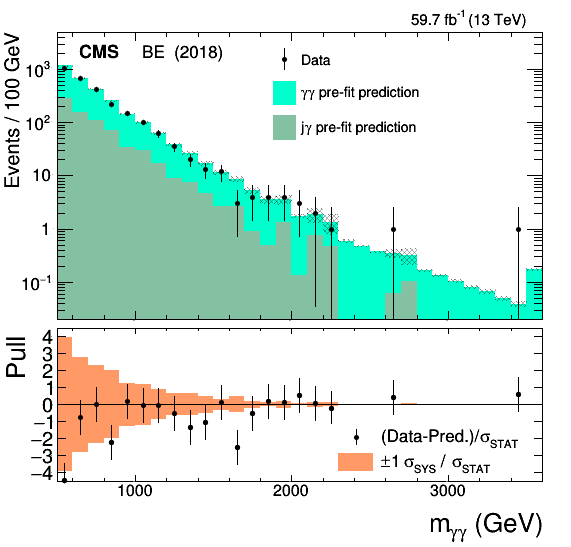
\includegraphics[width=0.49\textwidth]{fig/PLOT_PRED_PULL_BE18_6000_ADDGRW_0_0.png}
}
\caption{The \mgg spectra in the prefit estimate for 2016; left the BB and right the BE channels.
These are the six observables used in the fit.
The final prediction is derived from a fit to the data, a procedure which absorbs residual mismodeling present at these plots.
}
\label{fig:Prefit_spectra2016}}
\end{figure}

\begin{figure}[!htbp]{\centering{
% 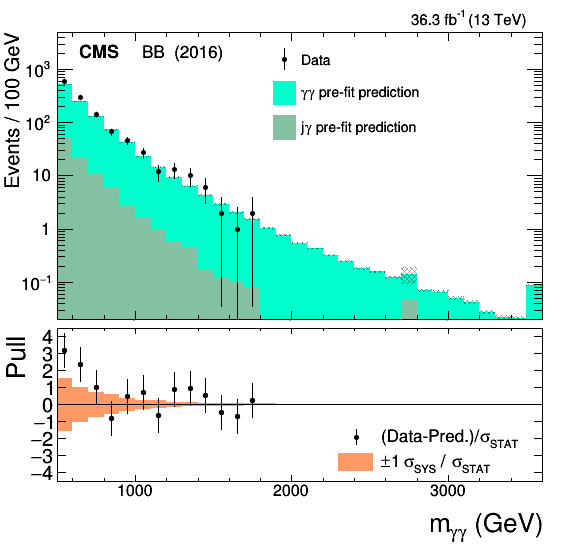
\includegraphics[width=0.49\textwidth]{fig/PLOT_PRED_PULL_BB16_6000_ADDGRW_0_0.png}
% 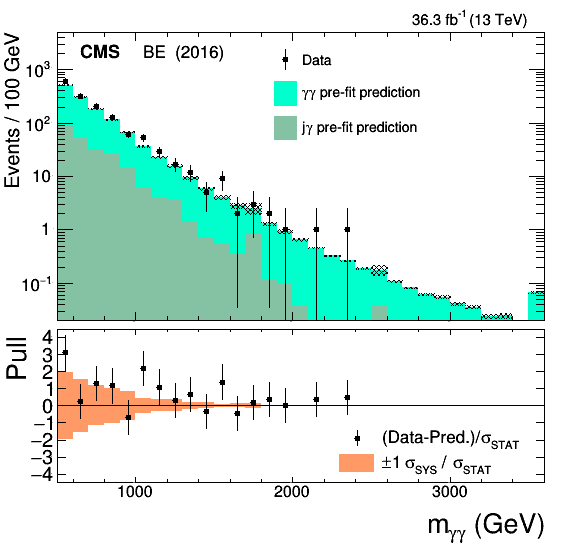
\includegraphics[width=0.49\textwidth]{fig/PLOT_PRED_PULL_BE16_6000_ADDGRW_0_0.png}
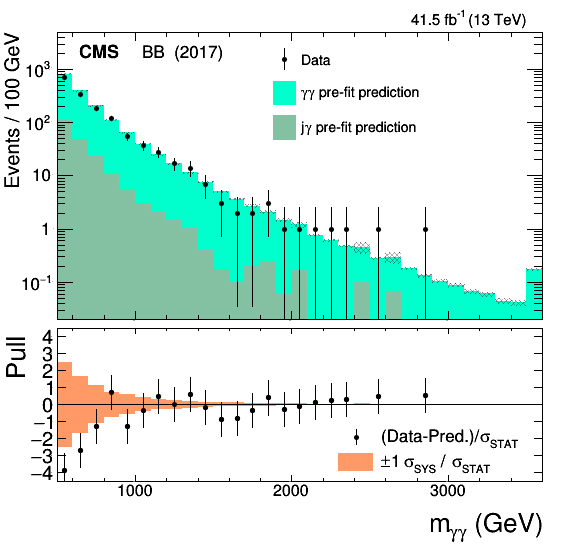
\includegraphics[width=0.49\textwidth]{fig/PLOT_PRED_PULL_BB17_6000_ADDGRW_0_0.png}
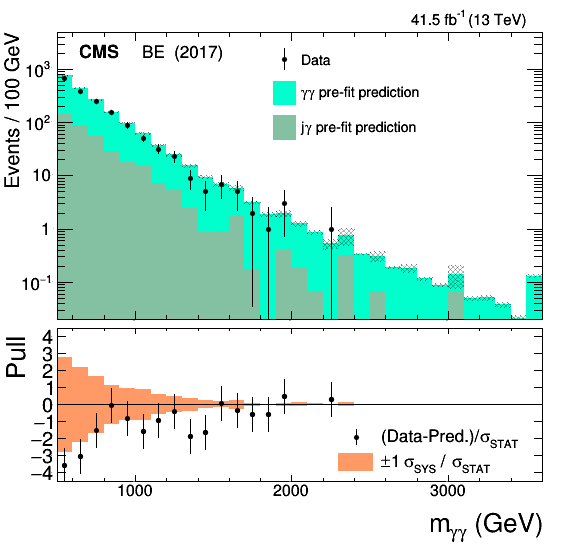
\includegraphics[width=0.49\textwidth]{fig/PLOT_PRED_PULL_BE17_6000_ADDGRW_0_0.png}
% 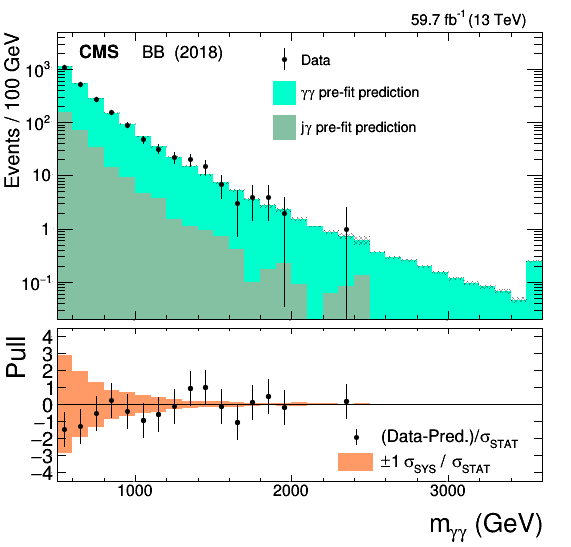
\includegraphics[width=0.49\textwidth]{fig/PLOT_PRED_PULL_BB18_6000_ADDGRW_0_0.png}
% 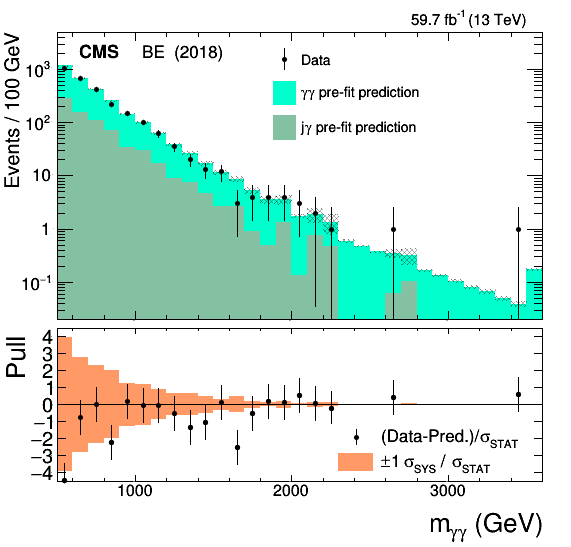
\includegraphics[width=0.49\textwidth]{fig/PLOT_PRED_PULL_BE18_6000_ADDGRW_0_0.png}
}
\caption{The \mgg spectra in the prefit estimate for 2017; left the BB and right the BE channels.
These are the six observables used in the fit.
The final prediction is derived from a fit to the data, a procedure which absorbs residual mismodeling present at these plots.
}
\label{fig:Prefit_spectra2017}}
\end{figure}

\begin{figure}[!htbp]{\centering{
% 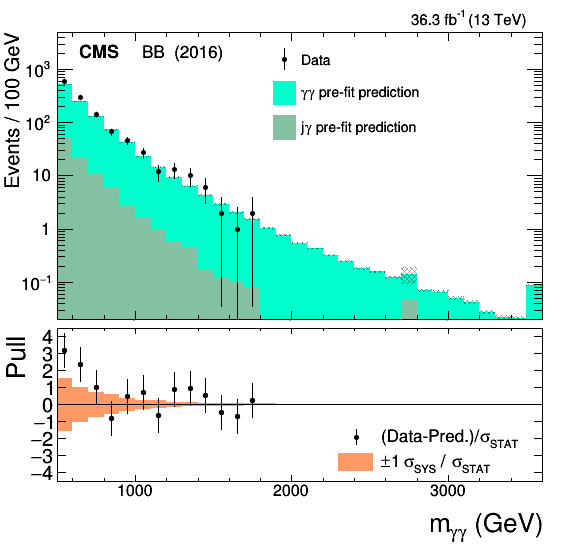
\includegraphics[width=0.49\textwidth]{fig/PLOT_PRED_PULL_BB16_6000_ADDGRW_0_0.png}
% 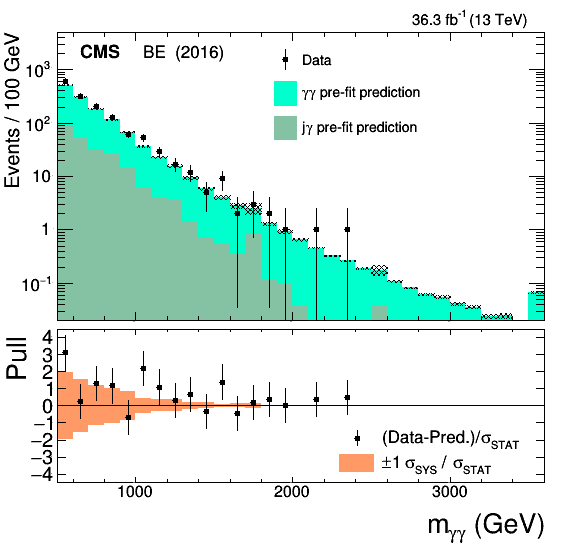
\includegraphics[width=0.49\textwidth]{fig/PLOT_PRED_PULL_BE16_6000_ADDGRW_0_0.png}
% 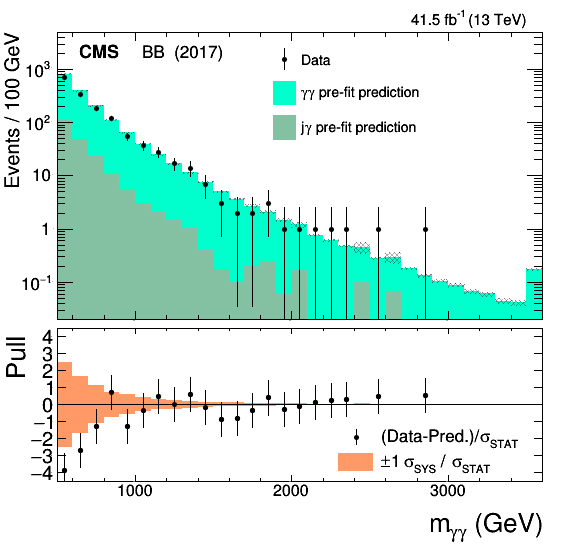
\includegraphics[width=0.49\textwidth]{fig/PLOT_PRED_PULL_BB17_6000_ADDGRW_0_0.png}
% 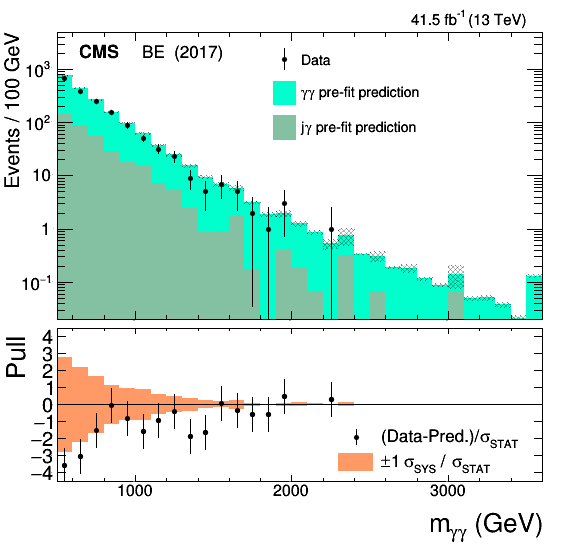
\includegraphics[width=0.49\textwidth]{fig/PLOT_PRED_PULL_BE17_6000_ADDGRW_0_0.png}
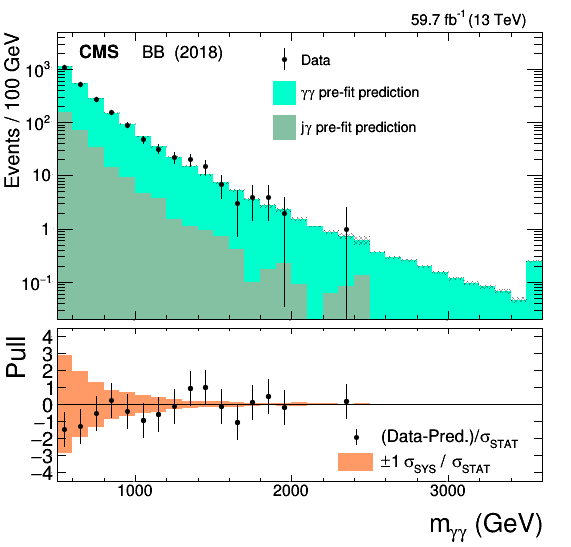
\includegraphics[width=0.49\textwidth]{fig/PLOT_PRED_PULL_BB18_6000_ADDGRW_0_0.png}
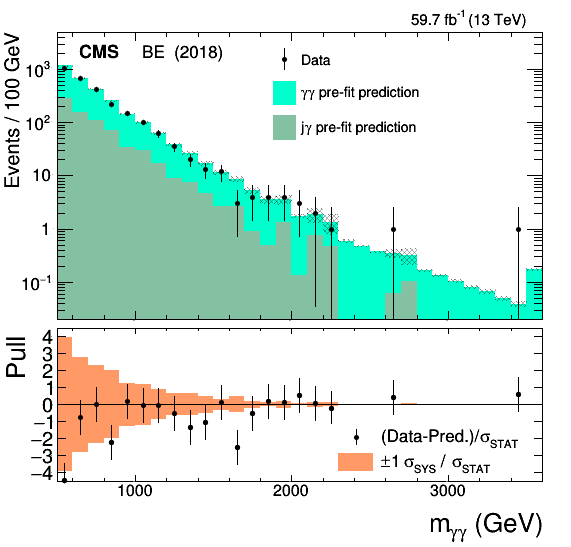
\includegraphics[width=0.49\textwidth]{fig/PLOT_PRED_PULL_BE18_6000_ADDGRW_0_0.png}
}
\caption{The \mgg spectra in the prefit estimate for 2018; left the BB and right the BE channels.
These are the six observables used in the fit.
The final prediction is derived from a fit to the data, a procedure which absorbs residual mismodeling present at these plots.
}
\label{fig:Prefit_spectra2018}}
\end{figure}

It is important to clarify at this point that the NNLO k-factor-corrected diphoton estimate together with the data-driven fake background estimate do not correspond to the final prediction of the total SM background. Instead, the final prediction is derived from the fit which simultaneously constrains nuisances and the signal strength. Additionally, the \mgg spectra presented in Figs.~\ref{fig:Prefit_spectra2016},~\ref{fig:Prefit_spectra2017}, and~\ref{fig:Prefit_spectra2018}  are the six observables used in the fit and termed as the prefit prediction together with all systematic uncertainties discussed in the previous Ch.~\ref{ch:systematics}. The nuisance parameters are then marginalized with the \THETA framework to derive posterior predictions for the \mgg spectra and signal strength, from which we can derive the 95\% CL exclusion limits on the BSM models probed. %ADD and clockwork models.


% For the limit setting, the \mgg spectra shown in figures ~\ref{fig:Prefit_spectra2016}, ~\ref{fig:Prefit_spectra2017}, ~\ref{fig:Prefit_spectra2018} are used. The six \mgg spectra are binned in 100 \GeV, starting at 500 \GeV and ending at 4000 \GeV. The last bin contains the overflow above that mass.
% For the continuum ClockWork model (CW) we start the fit from 1 \TeV (as we are constrained from the signal generation which results in fluctuations otherwise for lower than 1 \TeV masses).
% The nuisance parameters are simultaneously marginalized in a bayesian marginalization constrain fit, and a posterior prediction for the combined diphoton+fake \mgg spectra is produced using the data as a constraint. The signal strength for the ADD and CW models are given flat priors bounded below by zero. Although the \gmgm background normalization is allowed to float freely (within 5\%) in the BB and BE categories separately, the low-mass data will easily constrain those nuisance parameters.

% \begin{figure}[!htbp]{\centering{
% 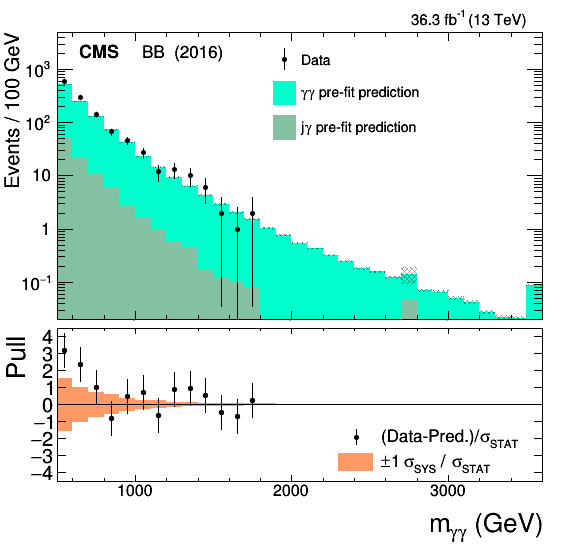
\includegraphics[width=0.49\textwidth]{fig/PLOT_PRED_PULL_BB16_6000_ADDGRW_0_0.png}
% 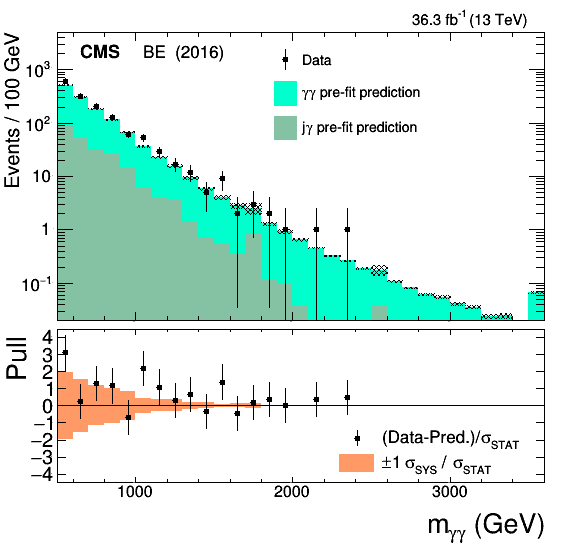
\includegraphics[width=0.49\textwidth]{fig/PLOT_PRED_PULL_BE16_6000_ADDGRW_0_0.png}
% 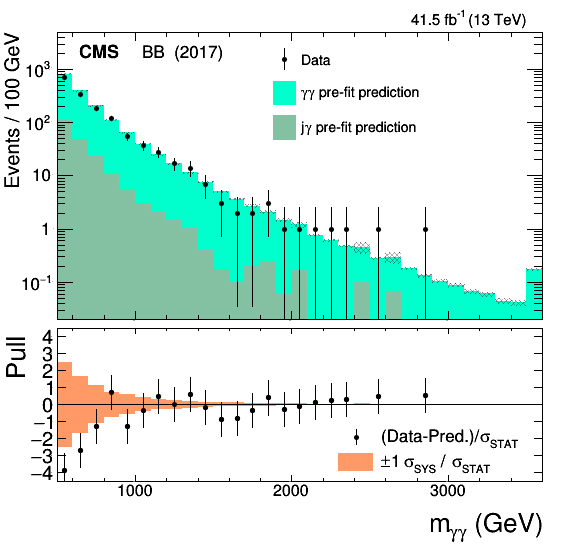
\includegraphics[width=0.49\textwidth]{fig/PLOT_PRED_PULL_BB17_6000_ADDGRW_0_0.png}
% 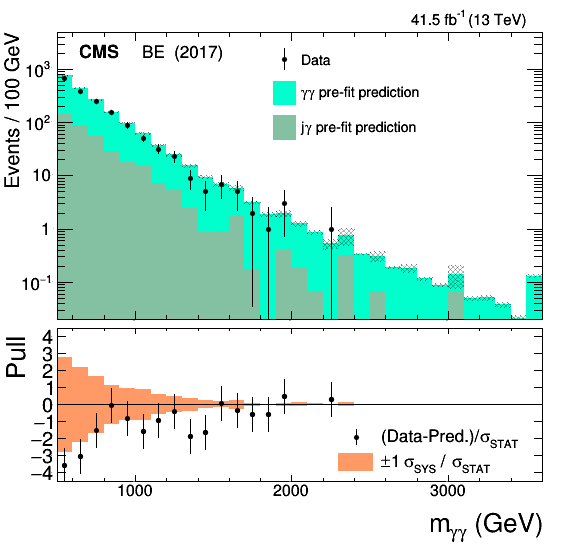
\includegraphics[width=0.49\textwidth]{fig/PLOT_PRED_PULL_BE17_6000_ADDGRW_0_0.png}
% 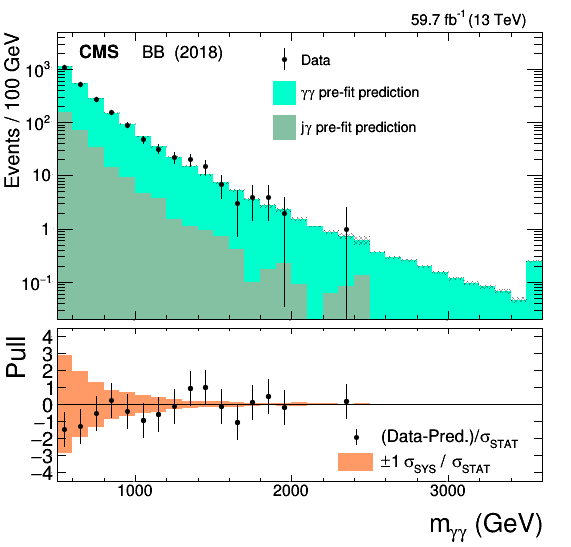
\includegraphics[width=0.49\textwidth]{fig/PLOT_PRED_PULL_BB18_6000_ADDGRW_0_0.png}
% 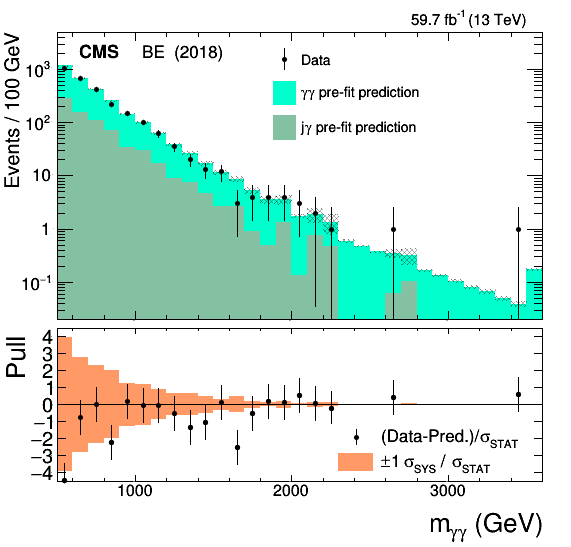
\includegraphics[width=0.49\textwidth]{fig/PLOT_PRED_PULL_BE18_6000_ADDGRW_0_0.png}
% }
% \caption{The \mgg spectra in the prefit estimate.
% Top to bottom: the 2016, 2017 and 2018 years; left the BB and right the BE channels.
% These are the six observables used in the fit.
% The final prediction is derived from a fit to the data, a procedure which absorbs residual mismodeling present at these plots.
% }
% \label{fig:Prefit_spectra}}
% \end{figure}



\subsection{Limits and Postfits}~\label{sec:postfitlimits}
After the marginalization procedure, \THETA returns postfit distributions, the nuisance postfit pulls, and the limits results for the models in question. In the next few pages, we will discuss more details on the shape-based analysis for the CW and ADD, respectively. In this shape-based approach there is a presupposition that the signal and background differ in their \emph{shape} and not only in the rate. A benefit from this procedure is that we are able to absorb and exploit higher-order corrections to the SM diphoton background prediction and their differences with the signal models.
% This approach presupposes that the signal and background differ in their \emph{shape} and not only in the rate.  
% A benefit we gain in this procedure is that we are able to absorb higher-order corrections to the diphoton prediction that are (in principle) unknown 
% directly into the background model under the assumption that those higher-order corrections result in a relatively flat k-factor.

Note that prior to unblinding the $\mgg$ region, we made use of pseudodata to run the full \textrm{THETA} limits machinery code and produce the expected results. The pseudodata are generated using the sum of the real $\gamma\gamma$ and fake $\gj$ and $jj$ spectra, which are the prefit background estimates, are used as the mean for poisson random number\footnote{https://root.cern.ch/doc/master/classTRandom.html#a1529ed28e6ce1230d135548460b12c19} generator from \ROOT. In this way, the pseudodata feature realistic systematic structures and fluctuations and we can check whether prefit pull trends are covered by our current parametrization. The results of the pseudodata used are found in Appendix~\ref{ch:appendix_pseudodata}.

\subsection{ADD Postfit results}~\label{sec:ADDPostfits}
 The ADD postfit results are shown in Figs.~\ref{fig:Postfit_Real2016ADD},~\ref{fig:Postfit_Real2017ADD},~\ref{fig:Postfit_Real2018ADD}, where we use light and dark blue for the real and fake background estimates respectively.
We observe from the bottom pads that various systematic trends initially present in prefit pulls are smoothened out in the postfit version. The post fit pulls exhibits only statistical fluctuations around one, and thus the \mgg parametrization absorbs the systematic effects. Figure \ref{fig:Postfit_Real_Inc} illustrates prefit and postfit results for all three years of data taking inclusively for the ADD scenario.

\begin{figure}[!htbp]{\centering{
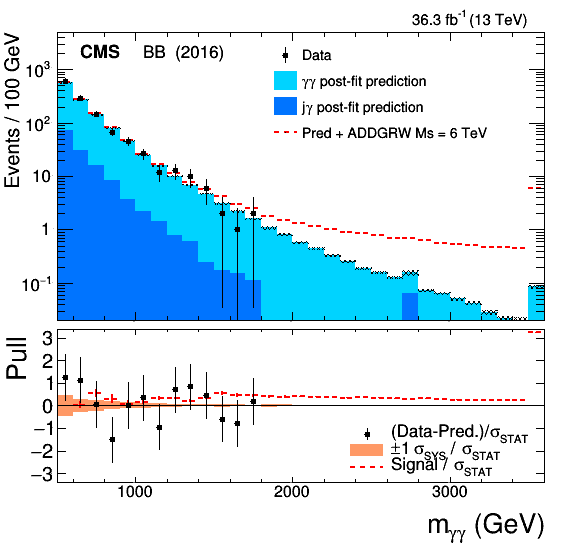
\includegraphics[width=0.49\textwidth]{fig/PLOT_PRED_PULL_BB16_6000_ADDGRW_1_0.png}
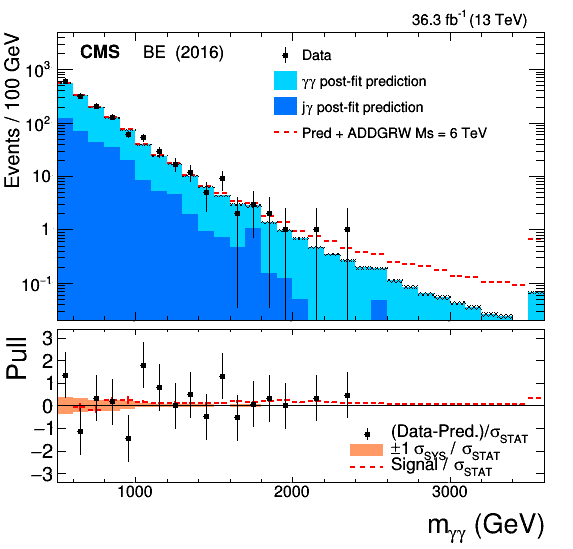
\includegraphics[width=0.49\textwidth]{fig/PLOT_PRED_PULL_BE16_6000_ADDGRW_1_0.png}
% 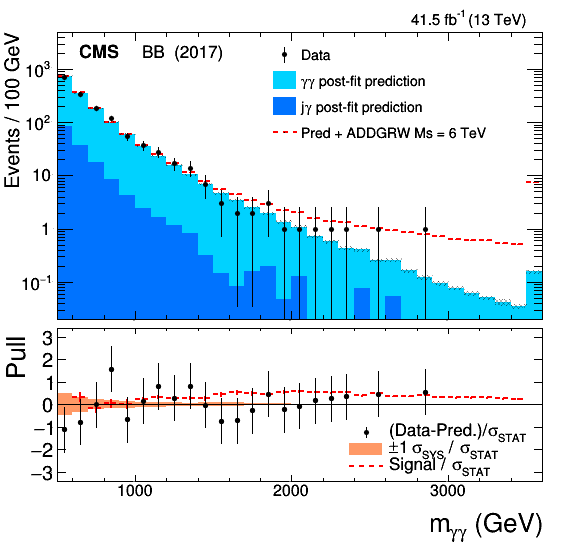
\includegraphics[width=0.49\textwidth]{fig/PLOT_PRED_PULL_BB17_6000_ADDGRW_1_0.png}
% 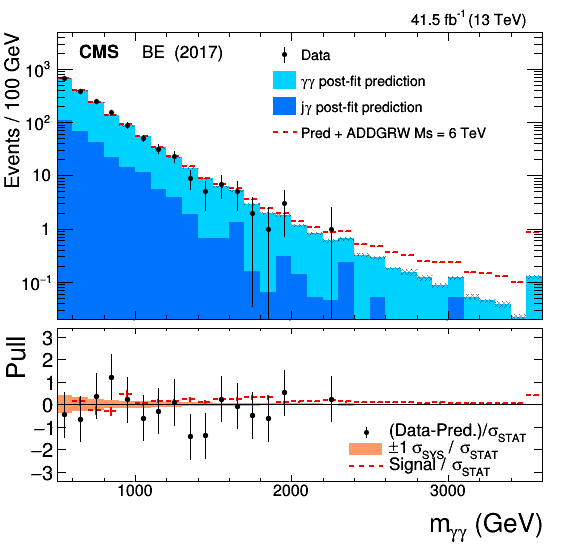
\includegraphics[width=0.49\textwidth]{fig/PLOT_PRED_PULL_BE17_6000_ADDGRW_1_0.png}
% 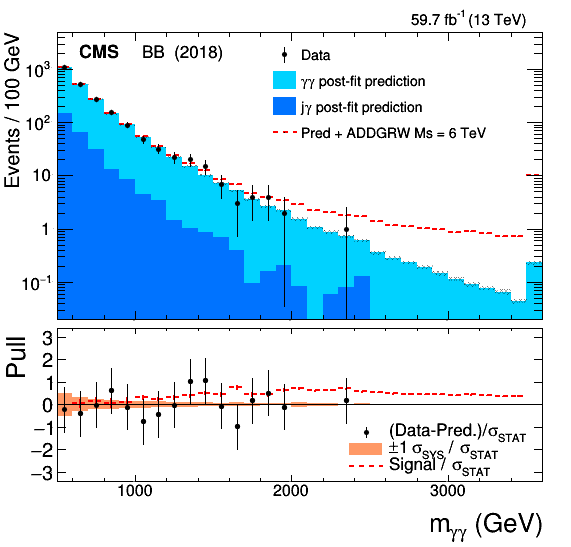
\includegraphics[width=0.49\textwidth]{fig/PLOT_PRED_PULL_BB18_6000_ADDGRW_1_0.png}
% 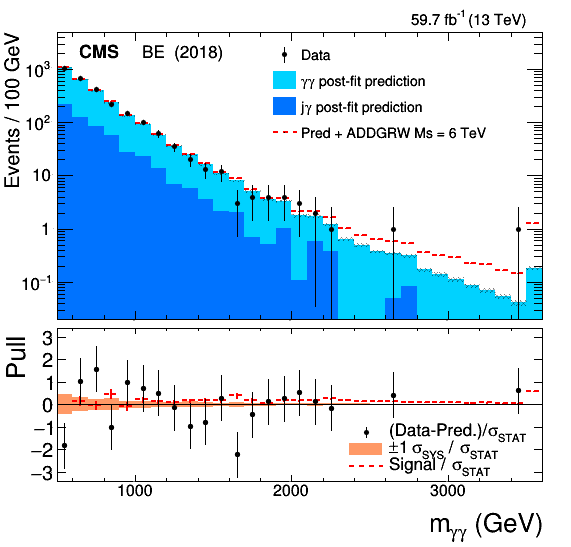
\includegraphics[width=0.49\textwidth]{fig/PLOT_PRED_PULL_BE18_6000_ADDGRW_1_0.png}  }
\caption{The ADD GRW postfit spectra (with real data) for BB (left) and BE (right) for 2016.}
\label{fig:Postfit_Real2016ADD} }
\end{figure}

\begin{figure}[!htbp]{\centering{
% 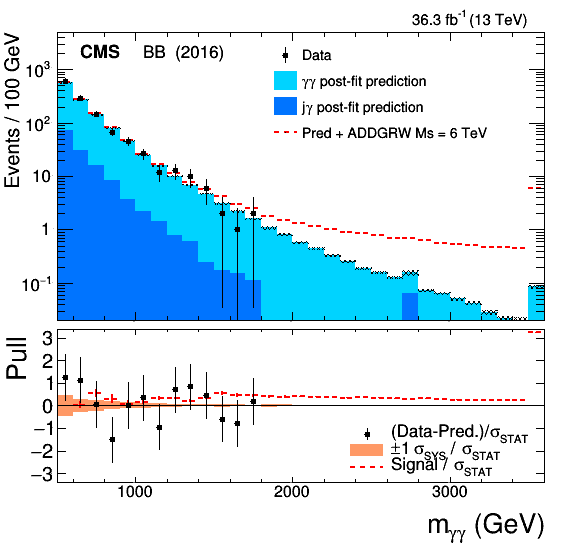
\includegraphics[width=0.49\textwidth]{fig/PLOT_PRED_PULL_BB16_6000_ADDGRW_1_0.png}
% 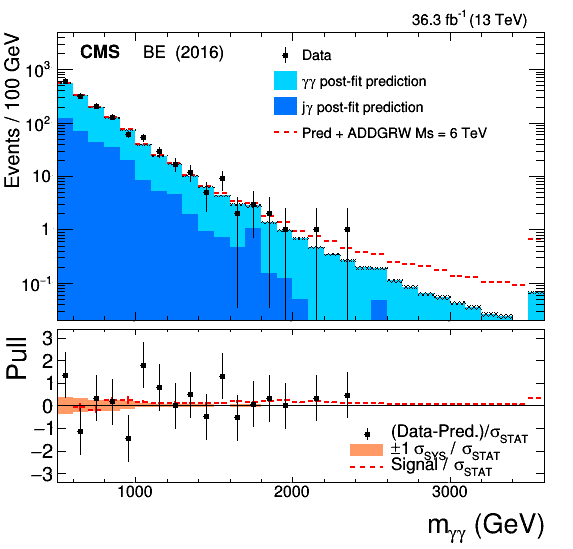
\includegraphics[width=0.49\textwidth]{fig/PLOT_PRED_PULL_BE16_6000_ADDGRW_1_0.png}
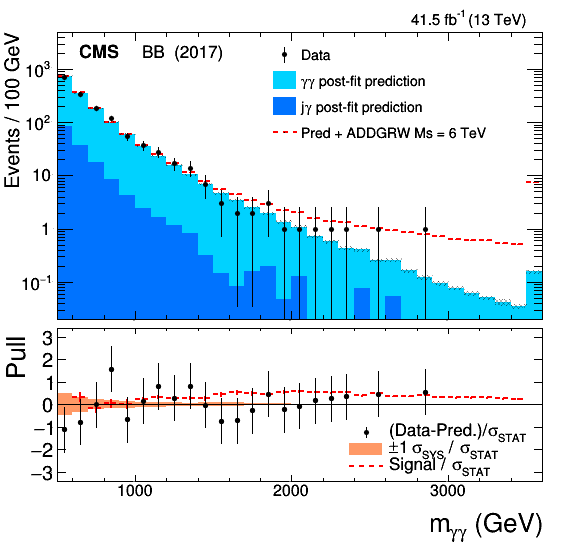
\includegraphics[width=0.49\textwidth]{fig/PLOT_PRED_PULL_BB17_6000_ADDGRW_1_0.png}
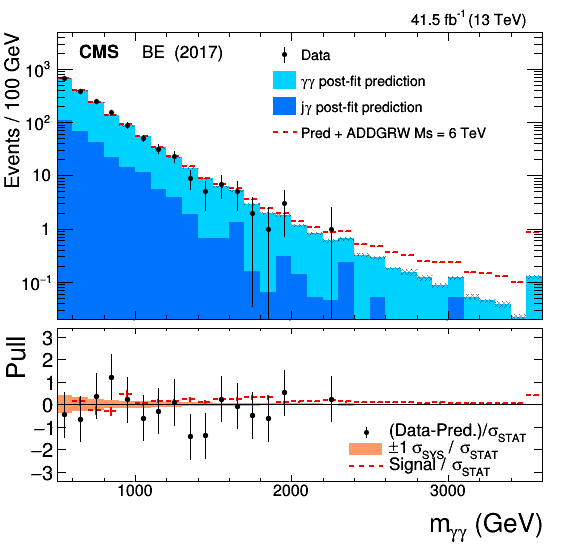
\includegraphics[width=0.49\textwidth]{fig/PLOT_PRED_PULL_BE17_6000_ADDGRW_1_0.png}
% 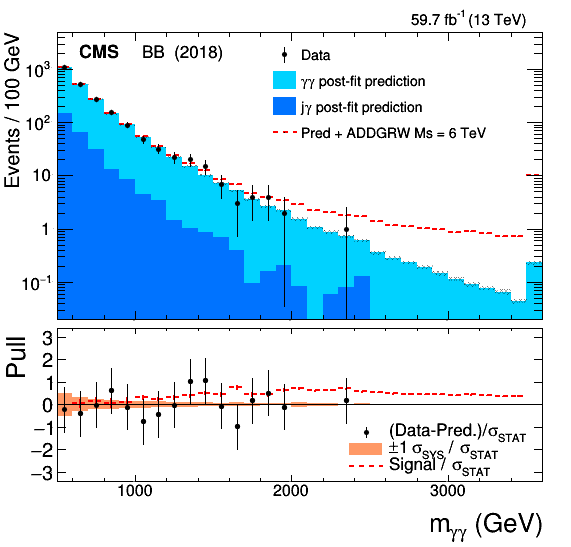
\includegraphics[width=0.49\textwidth]{fig/PLOT_PRED_PULL_BB18_6000_ADDGRW_1_0.png}
% 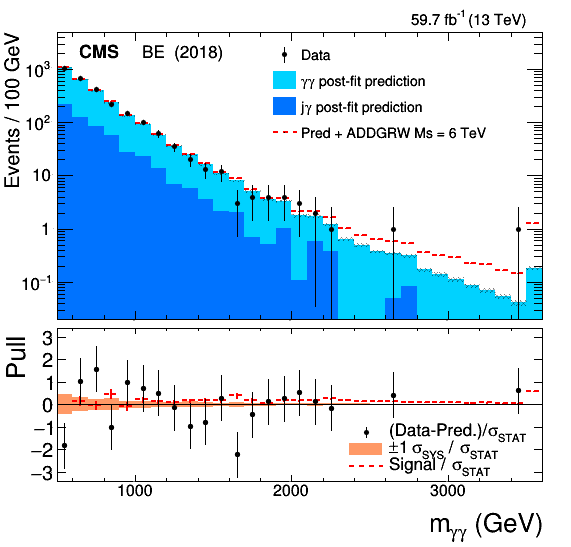
\includegraphics[width=0.49\textwidth]{fig/PLOT_PRED_PULL_BE18_6000_ADDGRW_1_0.png}  }
\caption{The ADD GRW postfit spectra (with real data) for BB (left) and BE (right) for 2017.}
\label{fig:Postfit_Real2017ADD} }
\end{figure}

\begin{figure}[!htbp]{\centering{
% 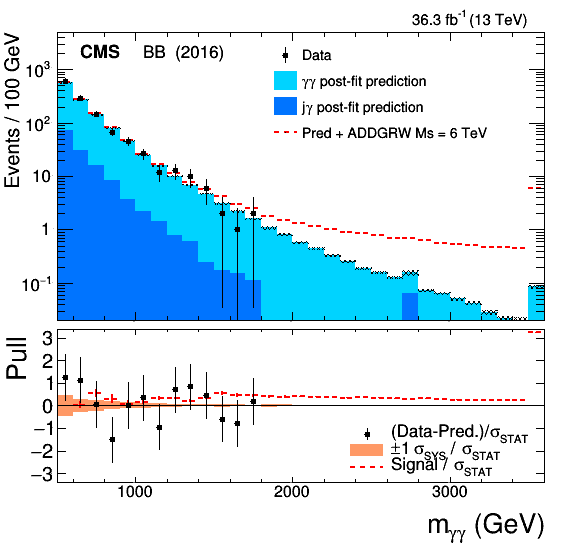
\includegraphics[width=0.49\textwidth]{fig/PLOT_PRED_PULL_BB16_6000_ADDGRW_1_0.png}
% 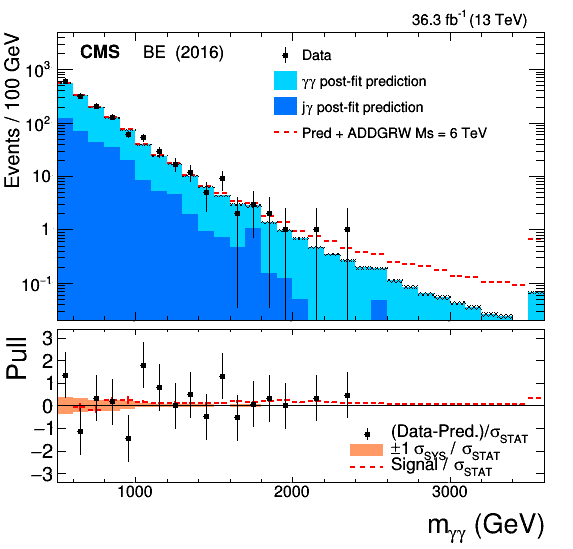
\includegraphics[width=0.49\textwidth]{fig/PLOT_PRED_PULL_BE16_6000_ADDGRW_1_0.png}
% 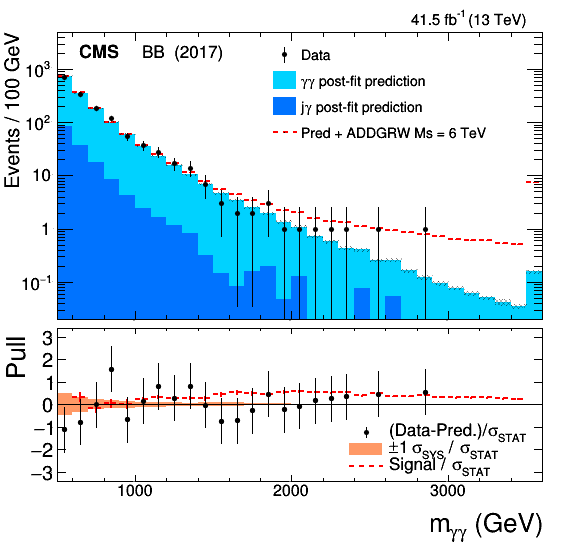
\includegraphics[width=0.49\textwidth]{fig/PLOT_PRED_PULL_BB17_6000_ADDGRW_1_0.png}
% 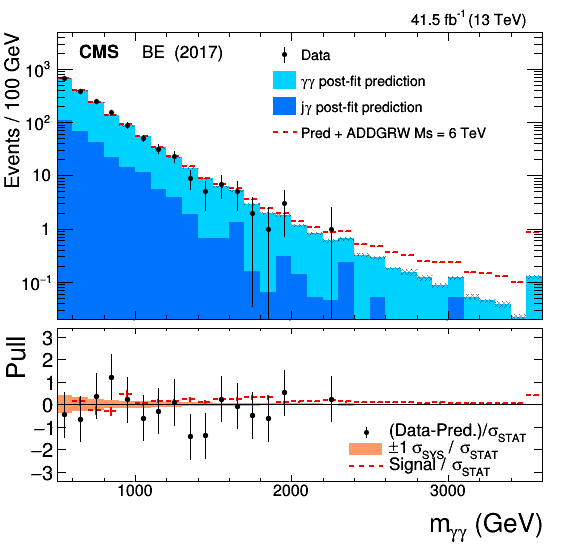
\includegraphics[width=0.49\textwidth]{fig/PLOT_PRED_PULL_BE17_6000_ADDGRW_1_0.png}
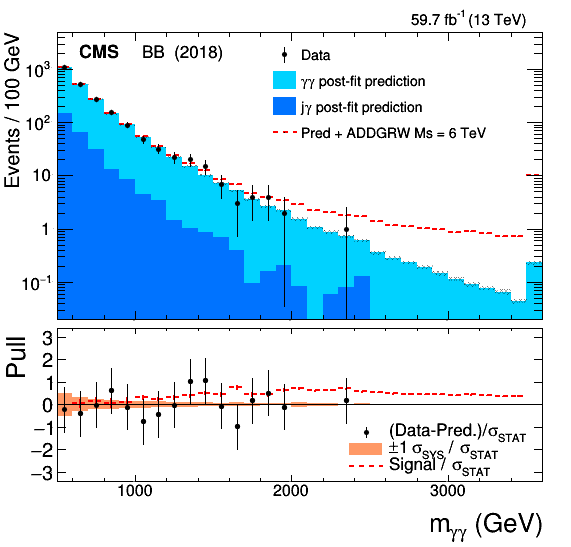
\includegraphics[width=0.49\textwidth]{fig/PLOT_PRED_PULL_BB18_6000_ADDGRW_1_0.png}
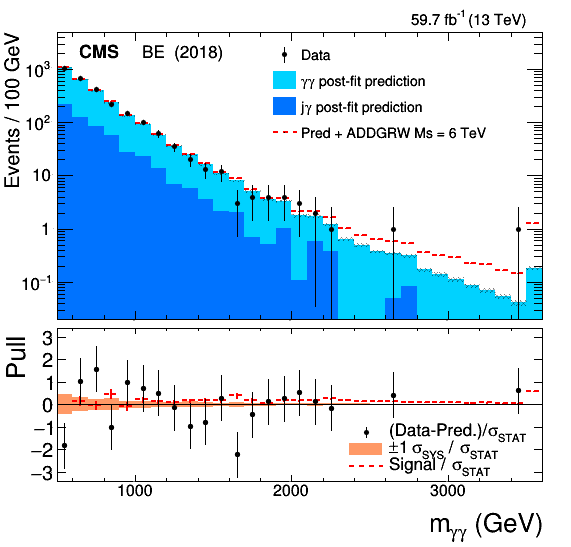
\includegraphics[width=0.49\textwidth]{fig/PLOT_PRED_PULL_BE18_6000_ADDGRW_1_0.png}  }
\caption{The ADD GRW postfit spectra (with real data) for BB (left) and BE (right) for 2018.}
\label{fig:Postfit_Real2018ADD} }
\end{figure}

\begin{figure}[!htbp]{\centering{
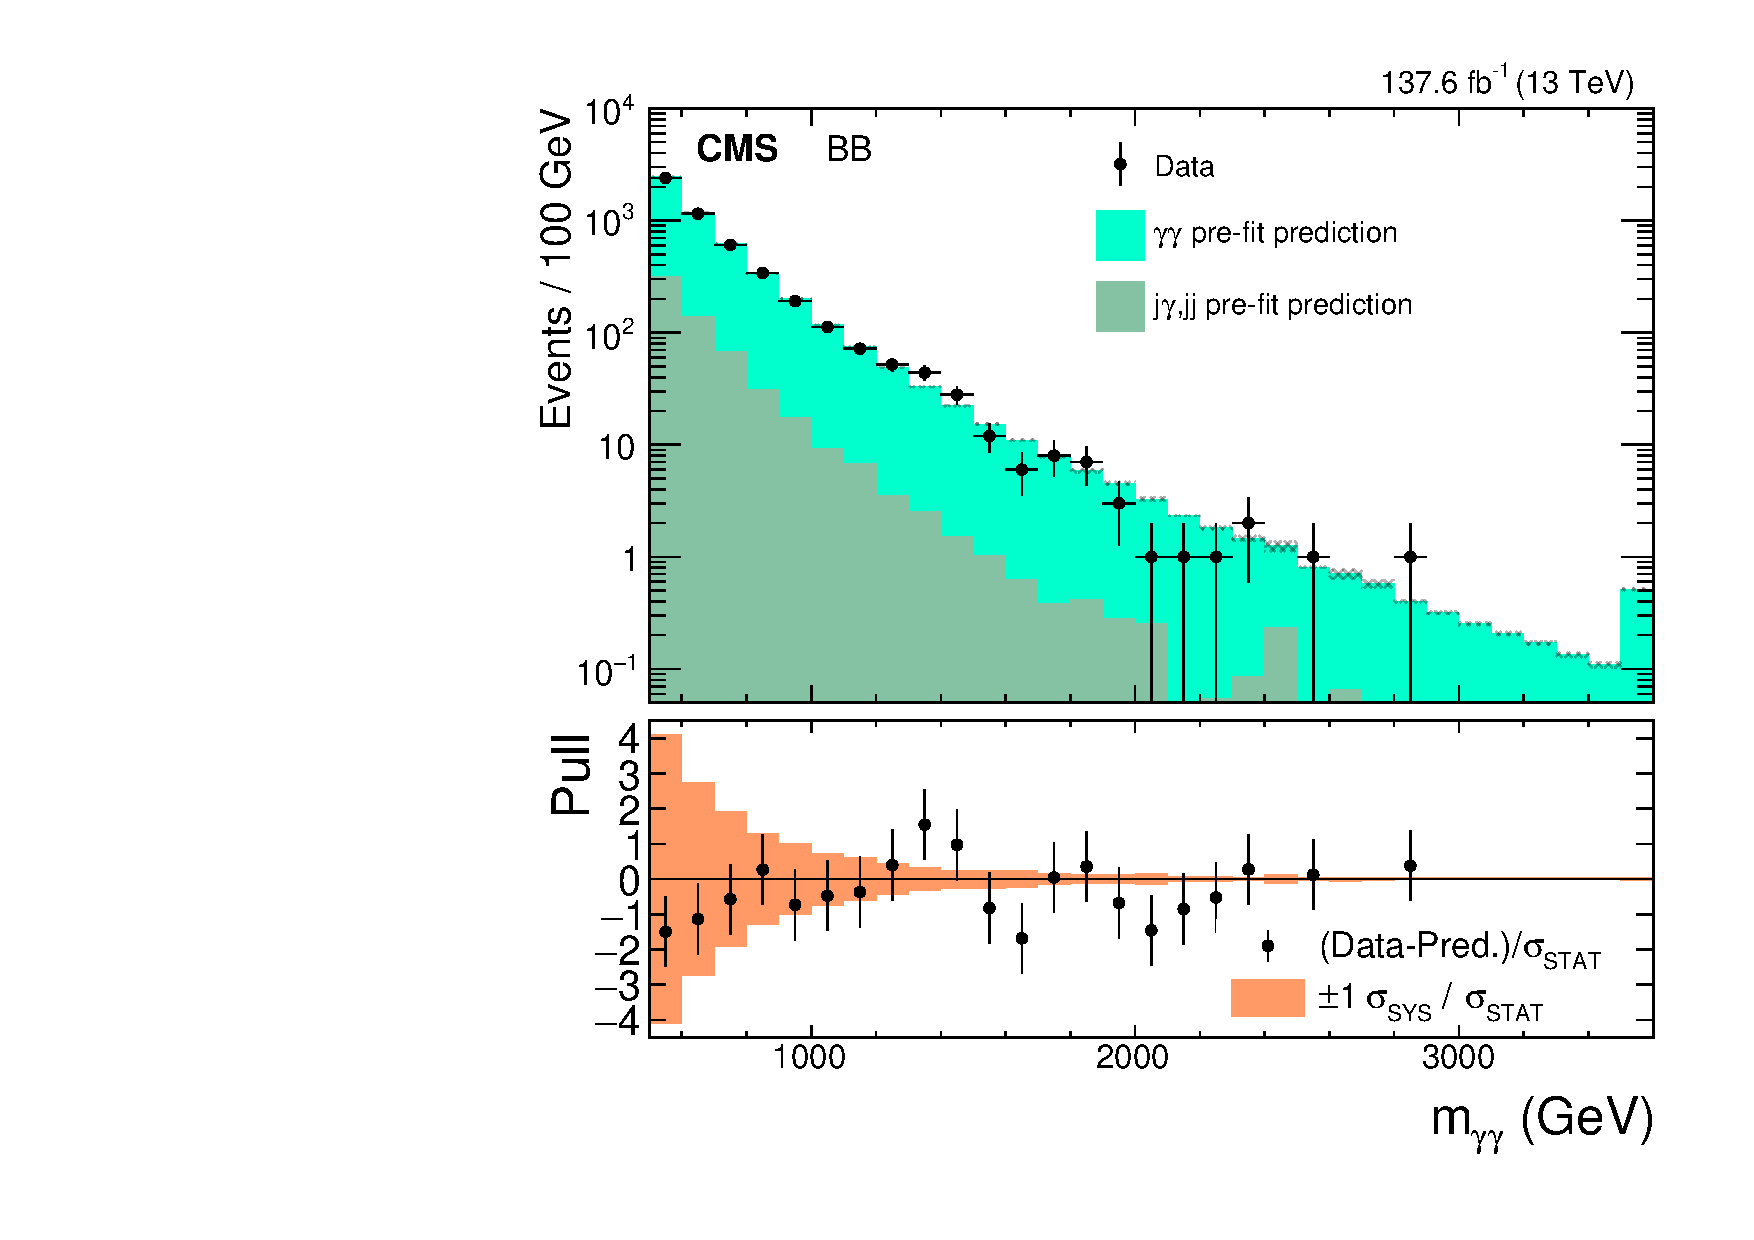
\includegraphics[width=0.49\textwidth]{fig/PLOT_PRED_PULL_BB161718_6000_ADDGRW_0_0.pdf}
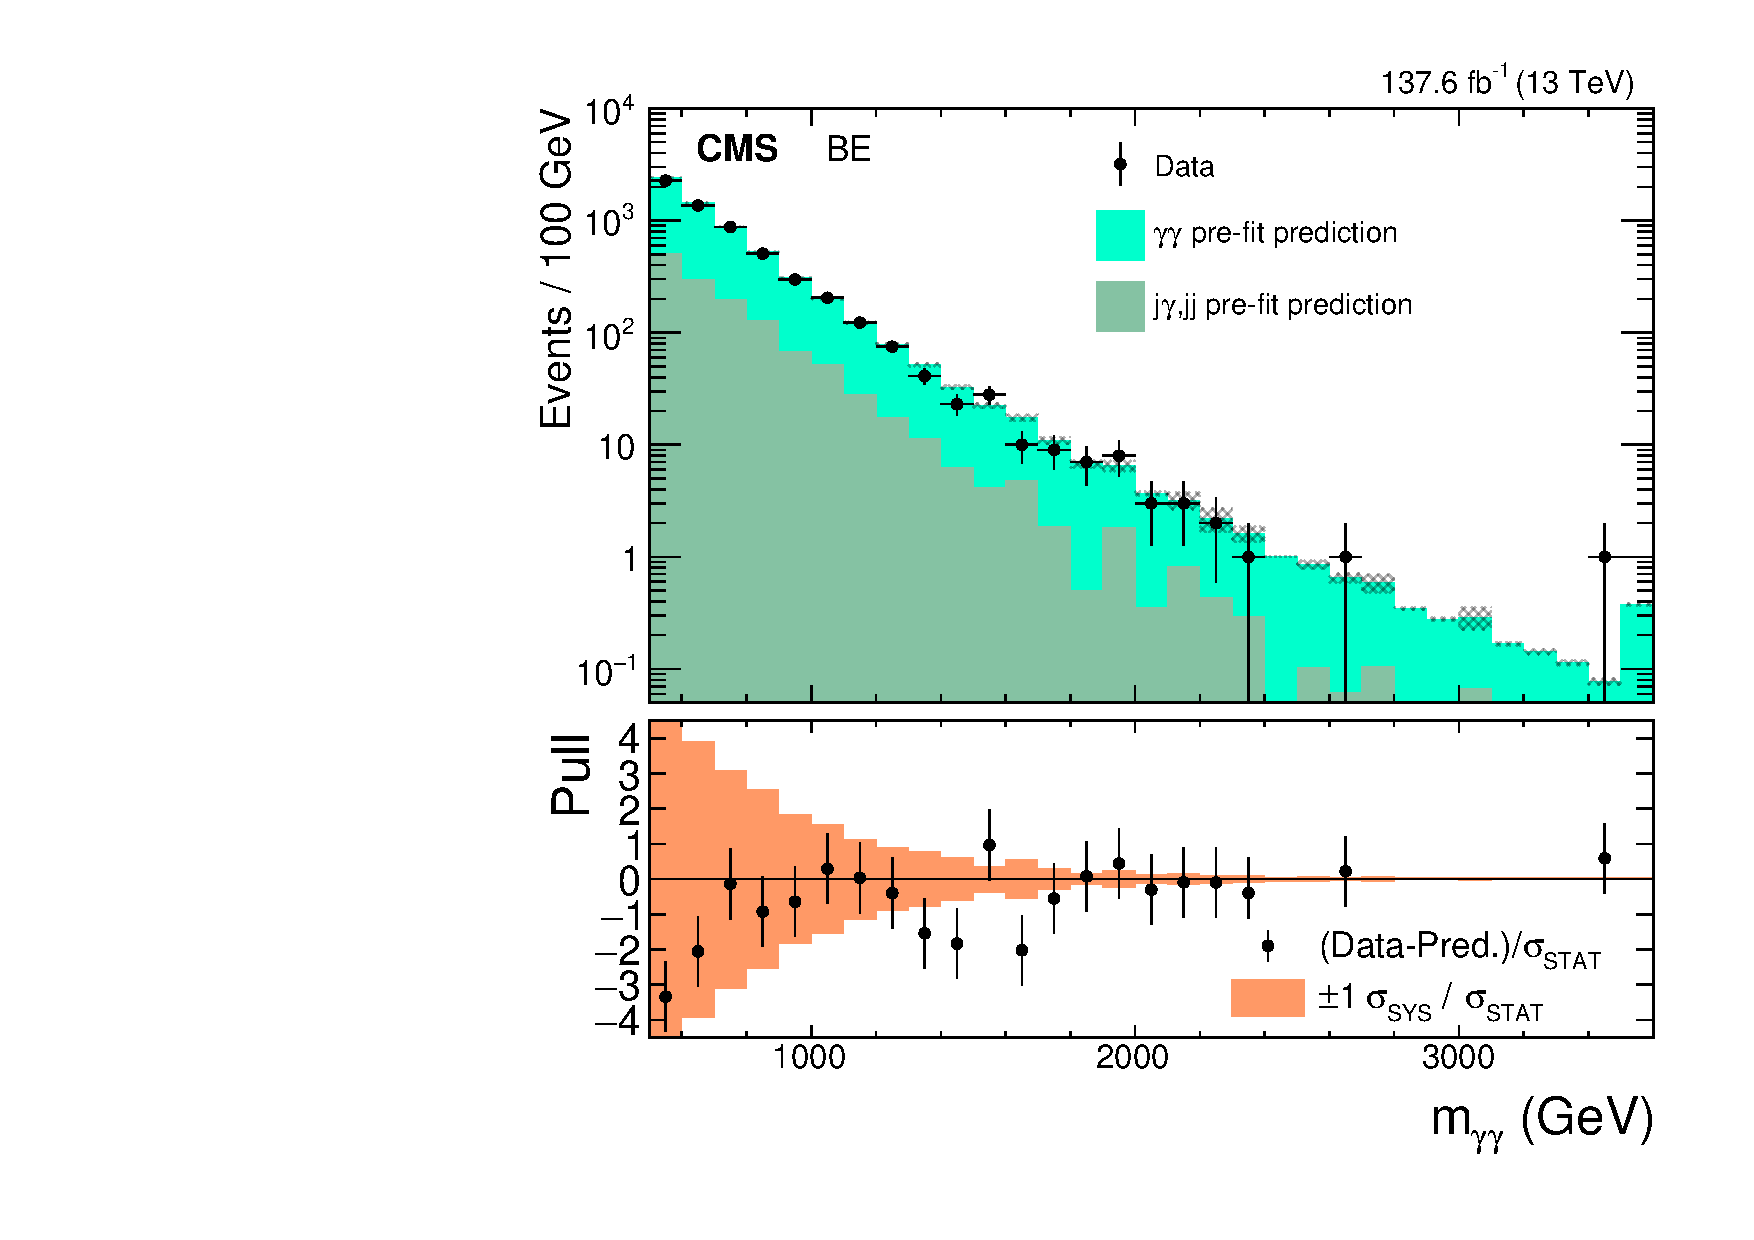
\includegraphics[width=0.49\textwidth]{fig/PLOT_PRED_PULL_BE161718_6000_ADDGRW_0_0.pdf}
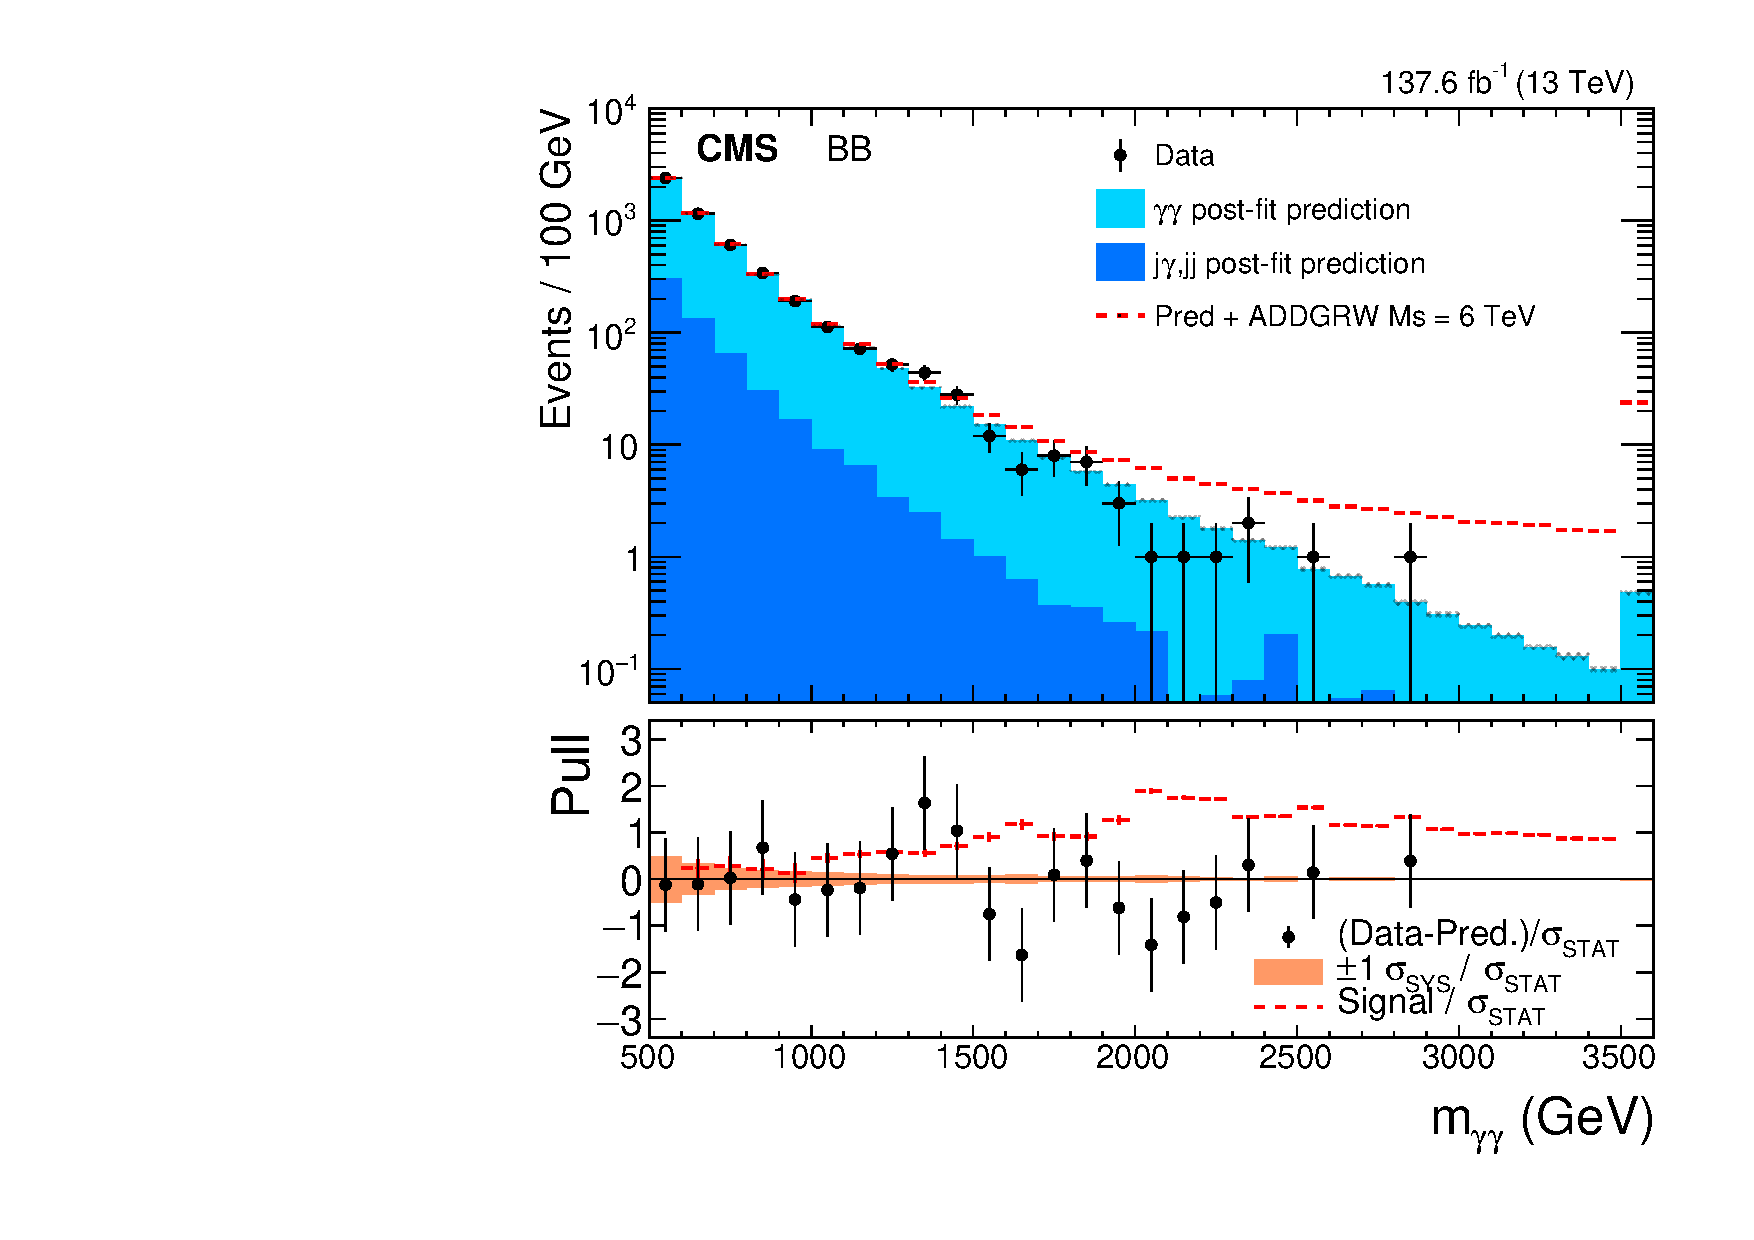
\includegraphics[width=0.49\textwidth]{fig/PLOT_PRED_PULL_BB161718_6000_ADDGRW_1_0.pdf}
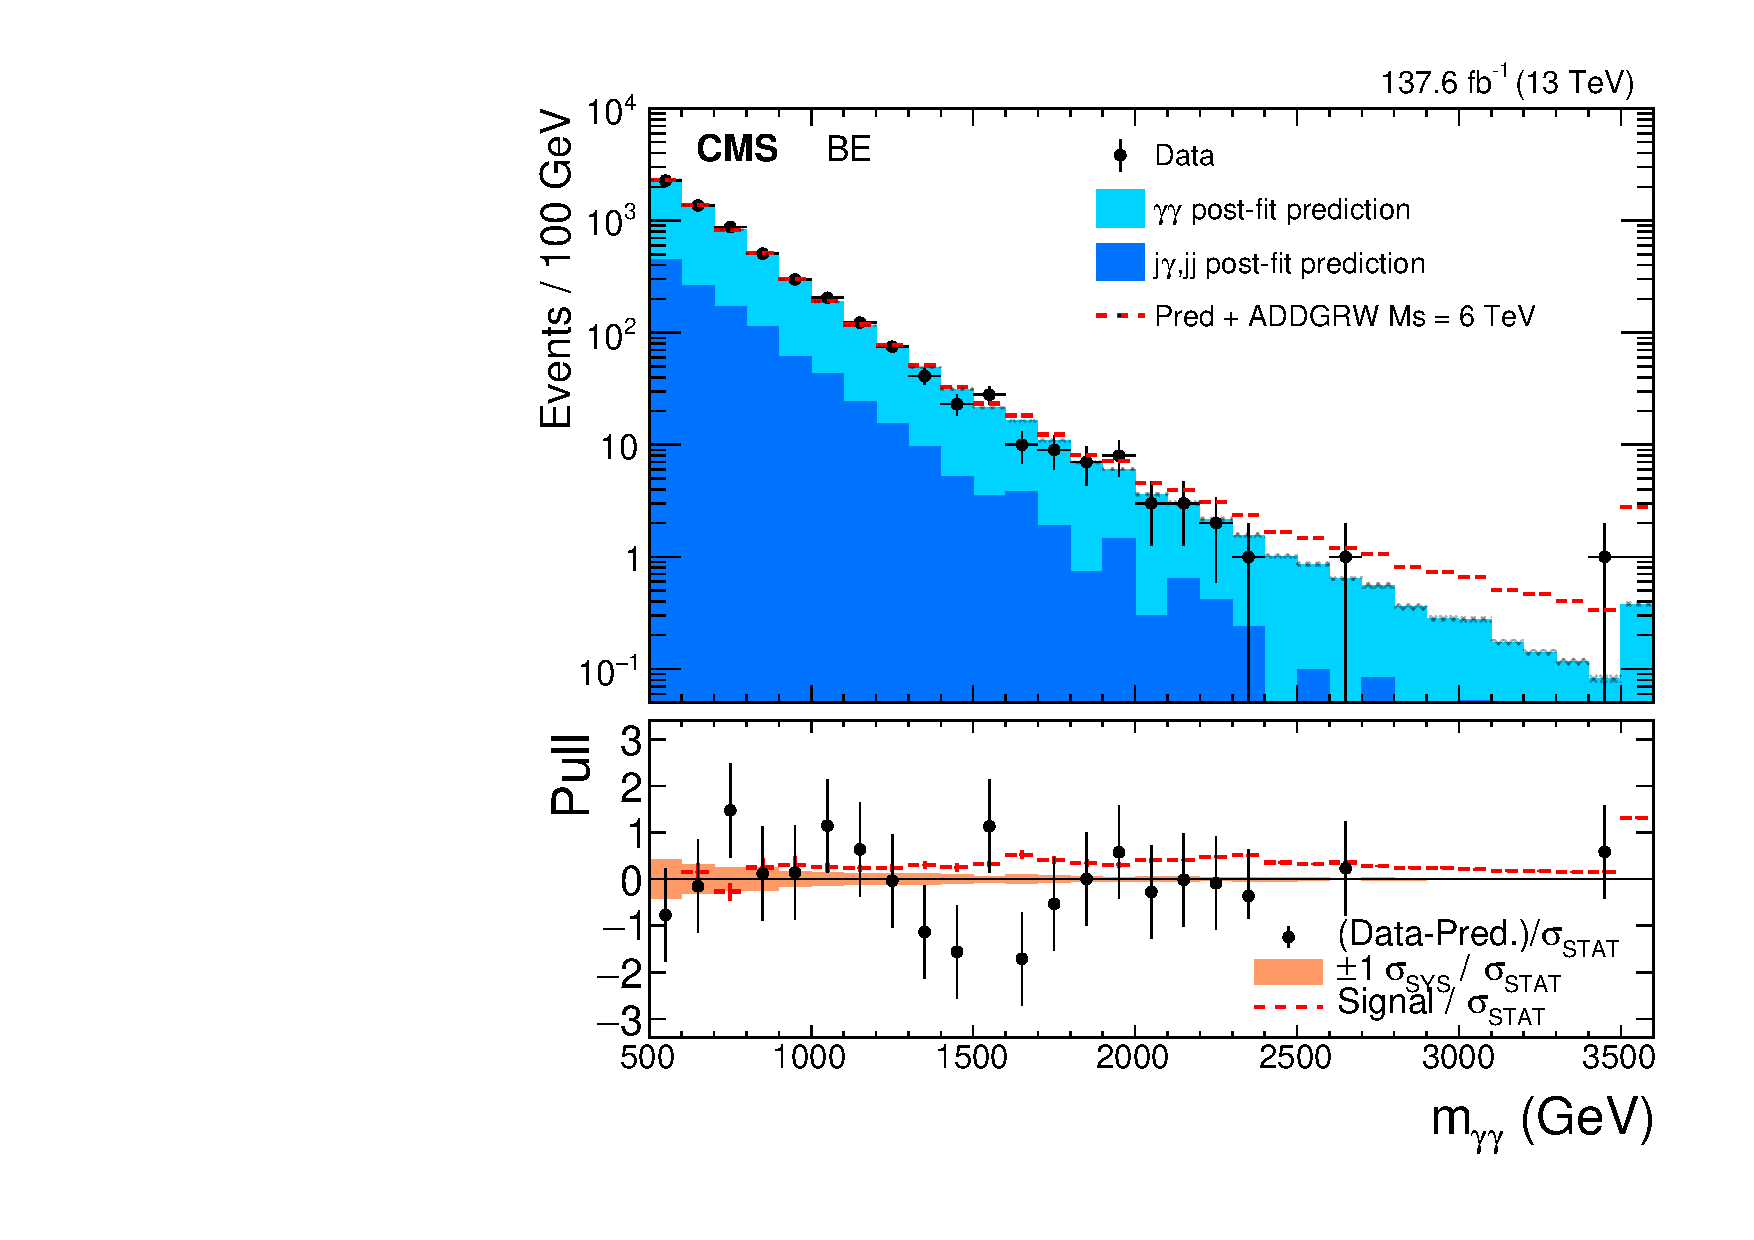
\includegraphics[width=0.49\textwidth]{fig/PLOT_PRED_PULL_BE161718_6000_ADDGRW_1_0.pdf}}
\caption{The prefit (top) and the postfit (bottom) spectra with real data for BB (left) and BE (right) for the three years of data taking inclusively. The plot shown in red at the bottom shows a representative signal plot for the ADD model with the GRW convention.}
\label{fig:Postfit_Real_Inc} }
\end{figure}


The nuisances are constrained and their priors which are either gaussian or lognormal probability distribution function transforms into their corresponding postfit version. While \COMBINE provides summary tables with the means and the standard deviations of the nuisances postfit pdfs, \THETA provides the full postfit pdfs spectra of each nuisance. The postfit probability distribution function (pdfs) of nuisances are presented in Figure~\ref{fig:Postfit_Nuisances_real}. In this figure, we see that signal strength named \texttt{beta\_signal} on the top-left, is strongly constrained near zero for GRW, $M_S=6\TeV$ as expected. Normalization nuisances of real \gmgm and fake $\gj,jj$ background events are constrained and their postfit pdfs are close to zero or some other value dictated by the fit on the data correcting prefit trends. The Postfit nuisances corresponding to the 50 pdfs of the PDFs nuisances; are all close to the prefit, that is it is a gaussian with mean zero and standard deviation of one, as this set of data can not constrain them further.

\begin{figure}[!htbp]{\centering{
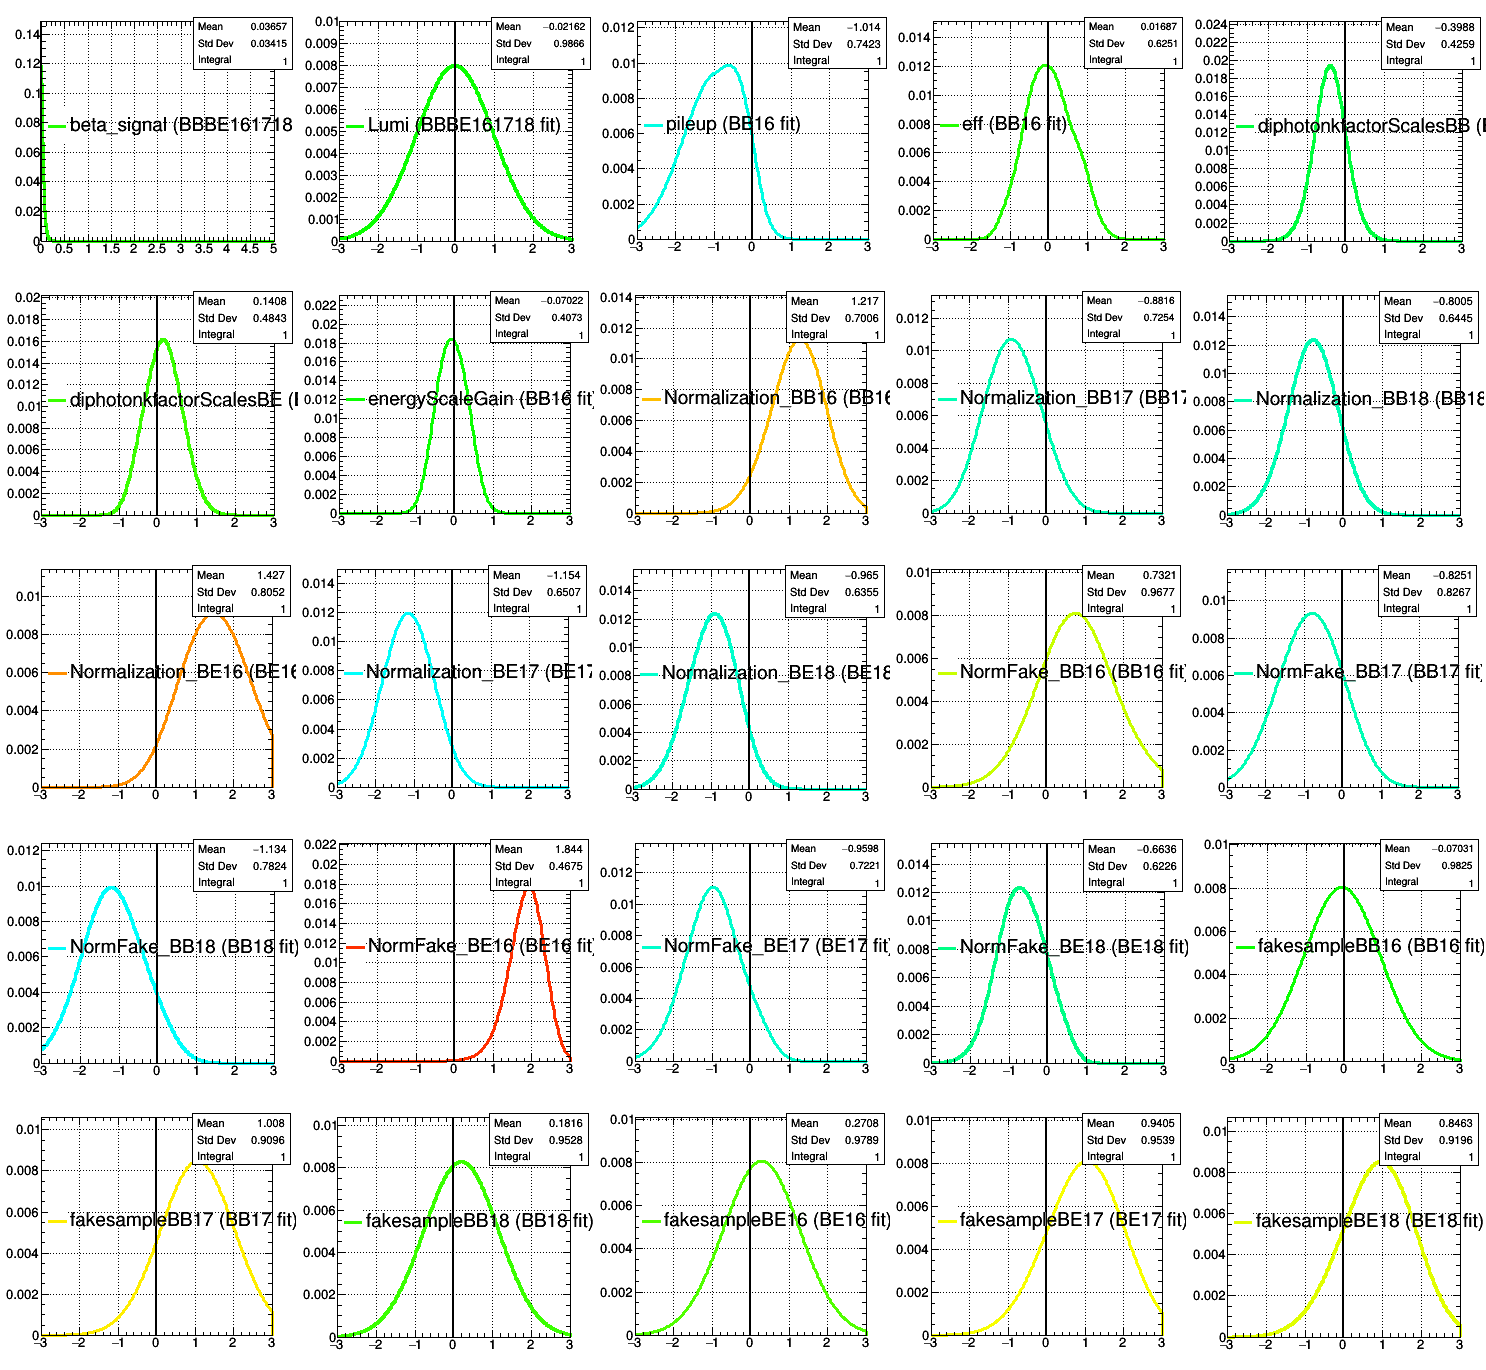
\includegraphics[width=1.0\textwidth]{fig/POST_All_BBBE161718_ADDGRW_real.png} }
\caption{The postfit probability distribution function (pdf) of each nuisance used in the six region fit.
Each plot corresponds to the sources (nuisances) presented of the table \ref{tab:Systematics} (names in labels).
The statistics panel of each plot contain the mean and the standard deviation of the pdf.
Text indicates the name of each nuisance, and the parenthesis after that indicates the regions in which this is constrained over (\ie{}, notes the correlations).
This information can also be found in table \ref{tab:Systematics}. }
\label{fig:Postfit_Nuisances_real} }
\end{figure}



\subsection{ADD Limits}~\label{sec:ADDlimits}
For the ADD model, we have the positive and the negative interference conventions which have significant shape differences. These are referred to as the GRW and Hewett- conventions respectively. We ran the limit code for all available $\Lambda_T$ values, which are equivalent to $M_s$ depending on the model convention. \THETA then provides us the upper limit on the signal strength at 95\% CL for each $M_S$ scenario. Instances of $M_s$ with postfit signal strength $<1$ are excluded at 95\% CL. The results for the ADD GRW model after fitting all six signal regions from BB16,..., BE18 are presented in Figure~\ref{fig:Limits_real}.
% We also plot the upper limit on signal strength vs the $M_S$ parameter in order to translate the upper limit on signal strength to lower limit on $M_S$. 

\begin{figure}[!htbp]{\centering{
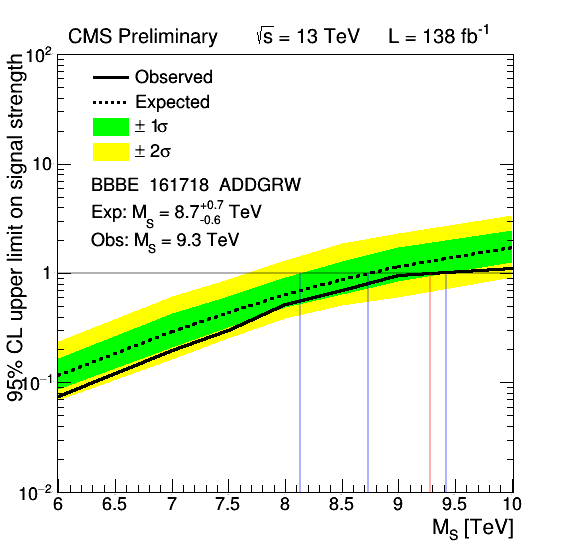
\includegraphics[width=0.49\textwidth]{fig/LIMITPLOT_BBBE161718_ADDGRW_real.png}
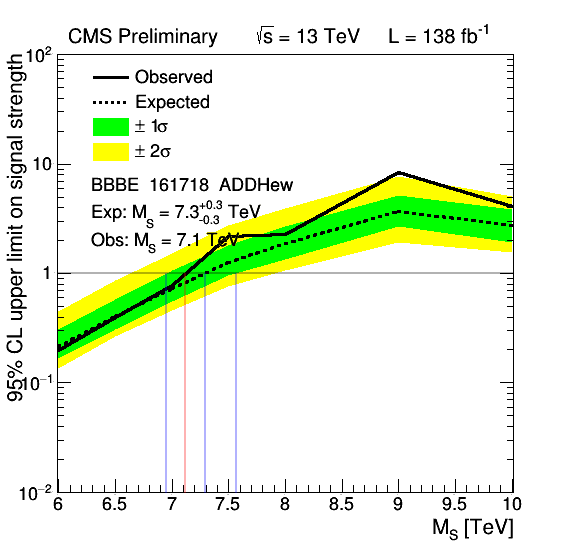
\includegraphics[width=0.49\textwidth]{fig/LIMITPLOT_BBBE161718_ADDHew_real.png}}
\caption{The 95\% CL limits on signal strength (y-axis) vs the $M_S$ (x-axis) and the limits on $M_S$ in legend for the ADD GRW model left, and Hewett negative right. These results are using real data. }
\label{fig:Limits_real}}
\end{figure}

From Figure~\ref{fig:Limits_real}, we can read the limits on the $M_S$ parameter as intersections with the horizontal line, where the signal strength is equal to 1. The green and yellow bands indicate the $\pm1\sigma$ and $\pm2\sigma$ standard deviation bands, respectively. The limits results from the GRW and Hewett- conventions could be translated to other ADD conventions as explained in Section~\ref{subsec:MC_Signal_ADD}. These are the HLZ conventions of positive interference for $n_{ED}=3,4,5,6,7$ which are obtained by scaling the GRW and the Hewett+ is obtained by scaling the Hewett- results. Table~\ref{Tab:Limits161718} presents the lower limits on $M_S$ scale for all available ADD signal scenarios.
\begin{table}[pt]
    \centering
    \caption{Exclusion limits on the mass scale \Ms (in units of {\TeVns}) for various conventions used in the calculation of the ADD large extra-dimensional scenario using the 2016-2018 CMS detector data corresponding to an integrated luminosity of 138 \fbinv. The total asymmetric uncertainties are shown on the expected limits.}
    \cmsTable{
    \begin{tabular}{ccccccccc}
        \\    
        \hline \hline
        \vspace*{-4.5mm} &&&&&&&& \\
        \multirow{2}{*}{Signal} & GRW & \multicolumn{2}{c}{Hewett} & \multicolumn{5}{c}{HLZ} \\
        & & negative & positive & $\nED=3$ & $\nED=4$ & $\nED=5$ & $\nED=6$ & $\nED=7$ \\ [\cmsTabSkip]
        \hline
        \vspace*{-2.5mm} &&&&&&&&& \\
        Expected & 8.7$^{+0.7}_{-0.6}$ & 7.3$^{+0.3}_{-0.3}$ & 7.8$^{+0.6}_{-0.5}$ & 10.3$^{+0.8}_{-0.7}$ & 8.7$^{+0.7}_{-0.6}$ & 7.9$^{+0.6}_{-0.5}$ & 7.3$^{+0.6}_{-0.5}$ & 6.9$^{+0.6}_{-0.5}$ \\ [\cmsTabSkip]
        Observed & 9.3 & 7.1 & 8.3 & 11.1 & 9.3 & 8.4 & 7.8 & 7.4 \vspace*{1.0mm} \\
        \hline \hline
    \end{tabular}
    }
    \label{Tab:Limits161718}
\end{table}
The limit code was previously tested with pseudodata and the results were consistent with the 2016 data search. With the unblinded results, we have set the most stringent limits on the ADD Large Extra dimensions in the diphoton channel.

The different trends that GRW and Hewett exhibit are artifacts that the former model predicts an excess while the latter deficit of events in high masses. As the data in the BB region where we are most sensitive indicate small deficit with respect to SM postfit estimate, observed limits behave this way in accordance with our expectations. 

% Plots in Figure~\ref{fig:Postfit_NuisancesPDFs} 
% Over all the postfit results presented in Figure \ref{fig:Postfit_Nuisances_real}--\ref{fig:Postfit_Real} suggest an expected "healthy" performance of the limit code and the fit. 

% In the following subsection we will present procedure of limits setting for the BSM models probed.
% The limits are set on signal strength for each of the individual signal scenarios presented in sec. \ref{subsec:MC_Signal_ADD}, (table \ref{table:ADDsamples} and Figure \ref{fig:ADDsignal}).

\subsection{CW Limits}~\label{sec:CWlimits}
The strategy for limit setting on the clockwork model (CW) is similar to the ADD model as described in the previous section. We use the data \mgg spectra to constrain the resonant excess due to the clockwork model by marginalizing over the aforementioned nuisance parameters assuming a flat prior for the signal strength. One difference with the ADD model is that for the CW we can only use the spectra $\mgg>1000$ \GeV. Since the CW distributions are combinations of the positive and negative interference ADD samples, we are constrained by the samples that are readily available. Below $\mgg>1000$ \GeV, statistical fluctuations dominate such that meaningful conclusions could not be made. 

From Eq.~\ref{eq:rescalingfactorCW}, we see that the CW signal strength normalization scales as $M_5^{-3}$, so a direct translation between an upper limit on the signal strength $\beta$ or in other references $\mu$, a lower limit on $M_5$ can be made for a fixed value of $k$. Figure~\ref{Fig:LIMIT_Clockwork_real} shows the 95\% CL exclusion in the $k$--$M_5$ plane with real data.
The signal shapes are generated for values of $k$ as low as 0.1 \GeV and up to 5 \TeV. The $k>M_5$ space is non-perturbative so we denote this region of phase-space with blue color in the $k$--$M_5$ plane.

\begin{figure}[h!]\centering
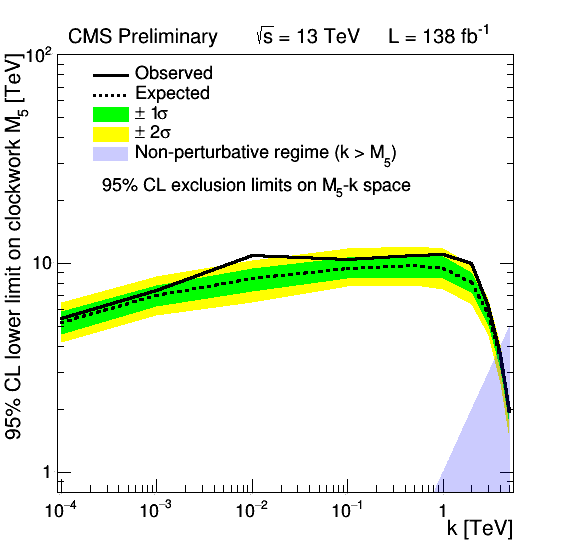
\includegraphics[width=0.49\linewidth]{fig/LIMITPLOT_BBBE161718_CWk_real.png}
\includegraphics[width=0.47\linewidth]{fig/LIMITPLOT_BBBE161718_CWk_nonLog_real.png}
\caption{The exclusion limit for the continuous graviton model in the clockwork framework (CW) over the $k-M_5$ parameter space. The shaded region denotes where the theory becomes non-perturbative. The right plot displays a non-log axis. }
\label{Fig:LIMIT_Clockwork_real}
\end{figure}

\begin{figure}[h!]\centering
\includegraphics[width=1.\linewidth]{fig/PRED_PRE_CWk_real.png}
\includegraphics[width=1.\linewidth]{fig/PRED_POST_CWk_real.png}
\caption{The CW prefit (top two rows) and the postfit (bottom two rows) \mgg spectra.
Columns left to right correspond to the years 2016, 2017, and 2018 respectively. }
\label{Fig:Postift_mgg_Clockwork_real}
\end{figure}

\begin{figure}[h!]\centering
\includegraphics[width=1.\linewidth]{fig/POST_All_BBBE161718_CWk_real.png}
\caption{The postfit pdfs for the 25 nuisance parameters used in the six SRs fit with CW model signal.}
\label{Fig:Postift_Nuisances_Clockwork_real}
\end{figure}


Figure~\ref{Fig:Postift_mgg_Clockwork_real} presents the \mgg spectra in the fitted range ($>1$ \TeV) in their prefit and postfit ranges. In these plots we also present the plain signal with the background unsubtracted so its shape is visible. We show the $k=1$ \TeV scenario in this plot which has a turn on at around 1 \TeV, thus the bulk of the signal events coincides with the bulk of the background. Similarly for $k<1$ \TeV, the signal events are spread in low masses and the sensitivity degrades as the shape difference with the SM background is small. For signal with $k\ge2$ \TeV the bulk of signal events are in high masses and in the overflow \mgg bin. The sensitivity is then limited by the statistics at the tails mostly at BB.

Figure \ref{Fig:Postift_Nuisances_Clockwork_real} present the postfit pdfs for the 25 nuisance parameters used in the six SRs fit with CW model as signal.
We observe that only a few of them are pulled to correct the prefit trends.
The pull effects are milder compared to the ADD as we fit $\mgg>1000~\GeV$ where the prefit is already in good agreement with the data.

% ~\footnote{https://github.com/cms-exotica-diphotons/diphoton-analysis/blob/phdClockwork/ClockworkAnalysis/scripts/makeCWHistos.C}

\subsection{\label{sec:ATLAS_results} Comparing CW results with ATLAS}
% Wait to write until after unblinding 

The CMS clockwork exclusion results shown in Figure~\ref{Fig:LIMIT_Clockwork_RUN1} show Run 1 results which excludes values of $M_5$ lower than 5 TeV for $k$ values in the range of 0.2 GeV to 2.0 TeV. With increased data in Run II, the limits were pushed further with values of $M_5$ lower than 5.5 TeV for k values from 0.1 to 2 TeV, and $M_5$ values lower than 11 TeV[8 TeV expected] to 1 TeV for $k$ values from 100 GeV to 5 TeV.  ATLAS~\cite{ATLAS:2023hbp}, have published their results on the CW model using a different signal generation and limit setting techniques. Figure~\ref{Fig:LIMIT_Clockwork_ATLAS} show that the ATLAS limits results without mass threshold is comparable results with ours.


\begin{figure}[h!]\centering
\includegraphics[width=0.47\linewidth]{fig/CWCMSI.png}
\caption{The previously published~\cite{cmsdiphoton2016} Run II, 2016-only 95\% CL exclusion limit for the continuous graviton model in the clockwork framework over the $k-M_5$ parameter space. The shaded bands represent the $\pm1$ and $\pm2$ standard deviation uncertainty in the expected limit. The shaded region in purple is where the theory becomes nonperturbative.}
\label{Fig:LIMIT_Clockwork_RUN1}
\end{figure}

\begin{figure}[h!]\centering
\includegraphics[width=0.9\linewidth]{fig/ATLASComp.png}
\caption{ATLAS~\cite{ATLAS:2023hbp} Run II exclusion limits with mass cut and without mass cut shown with flipped CMS results for comparative purposes.}
\label{Fig:LIMIT_Clockwork_ATLAS}
\end{figure}


\section{Preliminary Exclusion Limits on Unparticles}

For the Unparticles, we use a cut-and-count approach using the CLs prescription in \COMBINE. The inputs to \COMBINE are datacards which contain the details of the experiment such as the signal and the background yields above \mgg $>$ 2000 \GeV. 

The CLs Method~\cite{Junk:1999kv, Read:2002hq} is also known as the modified frequentist method which is more conservative than the standard p-value procedure. It is often used in particle physics experiments as the mathematical form shown in Eq.~\ref{eq:cls} avoids excluding a signal model when the sensitivity is low and also protects against exclusions due to underfluctations in the data. The CLs prescription takes the ratio of the p-values under signal plus background, $p_\mu$ and background-only $p_b$ hypotheses

\begin{equation}
\label{eq:cls}
    CL_s = \frac{p_{\mu}}{1-p_b}.
\end{equation}

To quickly estimate the expected limits we use the Asymptotics Limits statistical method which is implemented in the \COMBINE framework. 

\begin{figure}[tbp!]
% \begin{center}
\includegraphics[angle=0,width=1\textwidth]{fig/UnparticlesCountingExperiment.png}
% \end{center}
\caption{Limits on the Unparticles signal strength as a function of $\Lambda_{\mathcal{U}}$. The top plots show the Spin-0 case for $d_u$ = 1.1, 1.5, 1.9. The bottom shows the spin-2 case.}
\label{fig:UnparLimPlots}.
\end{figure}

For this preliminary study, we only make use of the 2017 centrally produced samples listed in Appendix~\ref{ch:appendix_signal_monte_carlo} and normalized them to the total 2016-2018 CMS luminosity. Table~\ref{tab:UnparLimitsPrelim} and Figure~\ref{fig:UnparLimPlots} show the preliminary limits results. Note that these expected limits results do not yet consider systematic uncertainties as well as the real data. 

\begin{table}[!htbp]
  \centering
  \caption{Preliminary limits on the Unparticles}
  \begin{tabular}{lll}
     & \textbf{Spin-0} & \textbf{Spin-2} \\
    $d_{\mathcal{U}}$ & $\Lambda_{\mathcal{U}}$ (TeV) & $\Lambda_{\mathcal{U}}$ (TeV) \\
    \hline
    1.1 & 7.8 & 2.7 \\
    1.5 & 2.5 & 2.4 \\
    1.9 & 2.2 & 2.5 \\
    \hline 
  \end{tabular}
  \label{tab:UnparLimitsPrelim}
\end{table}

\subsection{Potential sources of additional sensitivity}

We also performed additional sensitivity studies on the $U\rightarrow \gamma\gamma$ channel by looking at various parameters and kinematic variables. For these initial studies, we have used GEN-only events. From Figure~\ref{fig:UnparHistogSensitivity}, we can see that we are more sensitive to spin-2 than spin-0 if $\Lambda_u$ and $d_{u}$ are fixed.  
We also find in the same figure that for a fixed $d_{u}$ ($\Lambda_{u}$) the sensitivity goes up with lower(higher) values of $\Lambda_{u}$ ($d_{u}$). In future extensions of this work, we could conduct a multivariable analysis (MVA) or machine learning techniques to exploit other variables such as $cos\theta^*$. This could provide additional sensitivity to the Unparticles model in the diphoton channel.

\subsection{Comparison with Z+MET search}

The search for Unparticles have also been done in the Z + MET channel where the unparticle appears as the missing energy undetected by CMS. In the latest results from Ref.~\cite{CMS:2020ulv}, upper limits were set at 95\% CL on the cross section with $\Lambda_U$ = 15~\TeV. The observed (expected) limits are 0.5 (0.7) pb, 0.24
(0.26) pb, and 0.09 (0.07) pb for $d_u$ = 1, $d_u$ = 1.5, and $d_u$ = 2. These limits depend on the choice of $\lambda$ and $\Lambda_{u}$, as the cross section scales with the Wilson coefficient, $\frac{\lambda}{\Lambda_{u}}$, and here $\lambda =1$ is also chosen. To compare this with other results, future limit plots should show how how the limit varies with $d_u$. 

% \begin{figure}
%     \centering
%     \includegraphics[scale=0.7]{fig/Unparticles.png}
%     \caption{The 95\% CL upper limits on unparticle+Z~\cite{CMS:2020ulv} production cross section, as a function of the scaling dimension d. These limits apply to fixed values of the effective cutoff scale $\Lambda_U$ = 15 TeV and coupling $\lambda$ = 1 }
%     \label{fig:UnparZMET}
% \end{figure}



% ==========
% In the framework of the ADD model of extra dimensions, we use the fits to the pmiss
% T distribution
% to calculate limits on the number of extra dimensions n and the fundamental Planck scale MD.
% The cross section limit calculated as a function of MD for the case where n = 4 is shown in
% Figure 11. The limits on MD as a function of n are obtained, as shown in Figure 12. The observed
% (expected) 95% CL exclusion upper limit on the mass MD is 2.9–3.0 (2.7–2.8) TeV compared to
% earlier results of 2.3–2.5 (2.3–2.5) TeV
% ==========

% \begin{figure}[!htbp]
% 	\centering
%     \includegraphics[scale=0.38]{fig/UnparticlesSpinSensitivity.png}
% 	\caption{In red and blue are the spin-0 and spin-2, $\mathcal{U}\rightarrow \gamma\gamma$ histograms with the same $\Lambda_u = 1000$~\GeV and $d_{u} = 1.1$. The leading-order Standard Model Prompt Diphoton Background is shown in cyan. These are generator-only simulations.}
% 	\label{fig:UFixedLambdaFixedDu}
% \end{figure}

\begin{figure}[!htbp]
	\centering
% 	\includegraphics[scale=0.038]{fig/H2Bottle.JPG}
    \includegraphics[scale=0.34]{fig/UnparticlesSpinSensitivity.png}
    \includegraphics[scale=0.4]{fig/UnparticlesConstantLambda_U.png}
    \includegraphics[scale=0.4]{fig/UnparticlesConstant_du.png}
   
	\caption{
  In the top, the red and blue are the spin-0 and spin-2, $\mathcal{U}\rightarrow \gamma\gamma$ histograms with the same $\Lambda_u = 1000$~\GeV and $d_{u} = 1.1$.
 The middle plot shows various $d_u$ values with a fixed $\Lambda_u = 2500$~\GeV. On the bottom, is a plot that has a fixed $d_u = 1.8$~\GeV, and $\Lambda$ is varied. The leading-order Standard Model Prompt Diphoton Background is shown in cyan. These are generator-only simulations.}
	\label{fig:UnparHistogSensitivity}
\end{figure}

\begin{figure}[!htbp]
	\centering
% 	\includegraphics[scale=0.038]{fig/H2Bottle.JPG}
    \includegraphics[scale=0.4]{fig/cosThetaStar.png}
	\label{fig:UnparCosThetaStar}
 \caption{This figure shows $\cos \theta^*$ plots of $U\rightarrow \gamma\gamma$ versus the leading order SM only background (cyan). The right plot shows a different $d_u$ for spin-2, curved differently from the SM background.}
\end{figure}

% \begin{figure}[!htbp]
% 	\centering
% % 	\includegraphics[scale=0.038]{fig/H2Bottle.JPG}
%     \includegraphics[scale=0.8]{fig/UnparticlesConstant_du.png}
% 	\caption{For the spin-2 case, a fixed $d_{u}$, our sensitivity to the model goes up with lower values of $\Lambda_{U}$.}
% 	\label{fig:UFixedDu2}
% \end{figure}

% \begin{figure}[!htbp]
% 	\centering
% % 	\includegraphics[scale=0.038]{fig/H2Bottle.JPG}
    
% 	\caption{For the spin-2 case, a fixed $\Lambda_{u}$, our sensitivity to the model goes up with higher values of $d_{U}$.}
% 	\label{fig:UFixedLU}
% \end{figure}

% \begin{figure}[tbp!]
% \begin{center}
% \includegraphics[angle=0,width=0.33\textwidth]{fig/limitsSpin0_du1p1_plot.png}
% \includegraphics[angle=0,width=0.33\textwidth]{fig/limitsSpin0_du1p5_plot.png}
% \includegraphics[angle=0,width=0.33\textwidth]{fig/limitsSpin0_du1p9_plot.png}
% \includegraphics[angle=0,width=0.33\textwidth]{fig/limitsSpin2_du1p1_plot.png}
% \includegraphics[angle=0,width=0.33\textwidth]{fig/limitsSpin2_du1p5_plot.png}
% \includegraphics[angle=0,width=0.33\textwidth]{fig/limitsSpin2_du1p9_plot.png}
% \end{center}
% \caption{Counting Experiment Results}
% \label{fig:Counting Experiment Results}
% \end{figure}
